\documentclass[12pt,twoside]{article} 

\usepackage[hmarginratio=1:1]{geometry}

\usepackage{graphicx}
\usepackage[utf8]{inputenc}
%\usepackage{amsmath}
\usepackage{fancyhdr}


\title{Diseño y construcción de un sistema UAV}
\author{Jordi Pérez Talamino \and Jordi Rebull Mestres}
\date{\today}

\begin{document}

\pagestyle{fancy}

\fancyhead{}

\fancyhead[RE,LO]{\thepage}
\fancyhead[RO,LE]{Diseño y construcción de un sistema UAV}

\fancyfoot{}
\fancyfoot[C]{
\includegraphics[scale=0.3]{Imatges/etseib.png}}
\maketitle

\newpage

\tableofcontents

\newpage

\maketitle

	\section{Funcionamiento de un cuadricóptero}\label{sec:funcionamiento}
	
		Cualquier aeronave es capaz de realizar 3 posibles rotaciones alrededor de los 3 ejes de coordenadas con origen en el centro de gravedad de la aeronave (Figura \ref{fig:rotations}). 
		Estos 3 ejes son: el eje lateral, el longitudinal y el vertical, y las maniobras se llaman cabeceo (en inglés, pitch), alabeo (roll) y guiñada (yaw).
		
		
		Un cuadricóptero se propulsa mediante cuatro conjuntos motor-hélice denominados rotores, situados en los extremos de la aeronave.
		Cada rotor en funcionamiento produce sobre la aeronave un empuje y un par sobre su eje de rotación. 
		Por este motivo, se utilizan 4 rotores idénticos y se colocan en forma de cruz (Figura \ref{fig:quadrotorhover}), 
		donde dos de los rotores giran en un sentido, y los otros dos lo hacen en sentido opuesto.
		
		\begin{figure}
			\centering
			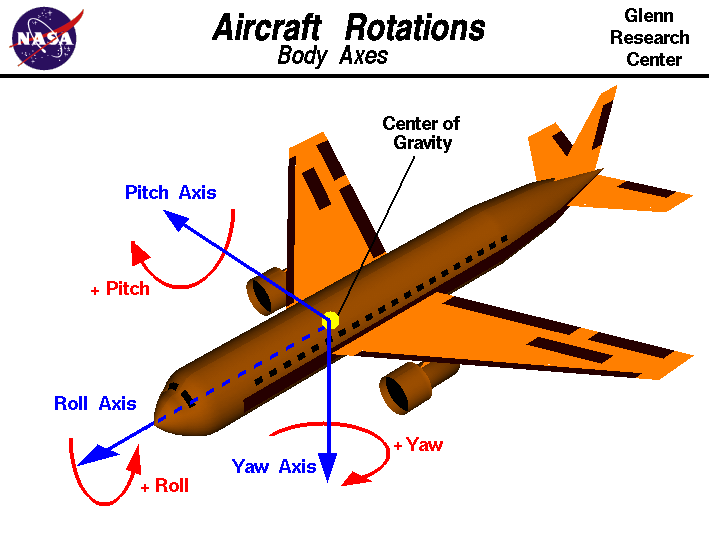
\includegraphics[width=0.7\textwidth]{Imatges/Funcionament/rotations.png}
			\caption{Rotaciones posibles}
			\label{fig:rotations}
		\end{figure}
		
		\begin{figure}
			\centering
			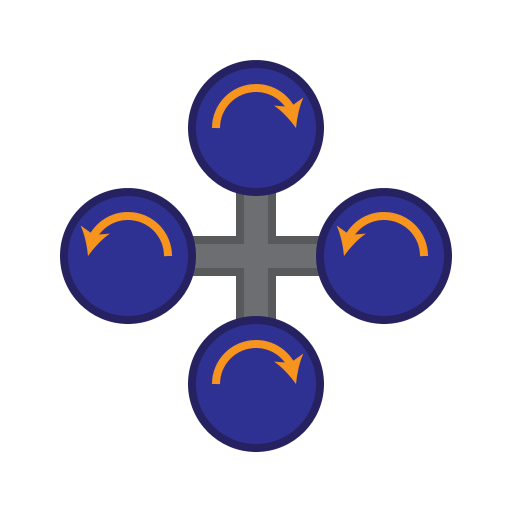
\includegraphics[width=0.4\textwidth]{Imatges/Funcionament/quadrotorhover.png}
			\caption{Distribución de los rotores en un cuadricóptero}
			\label{fig:quadrotorhover}
		\end{figure}
		
		Con esta conFiguración, si los 4 rotores giran con la misma velocidad angular, el par aerodinámico resultante sobre la aeronave es nulo, y entonces no hay aceleración angular en la dirección yaw. Así es como un quadricóptero se mantiene volando a una misma altitud y sin girar sobre si mismo, y acelerando o frenando por igual los 4 rotores es como gana o pierde altitud, respectivamente. 
		
		Para controlar el roll y el pitch, el cuadricóptero aumenta el empuje de un rotor y disminuye el empuje del rotor diametralmente opuesto (Figura \ref{fig:quadrotorpitch_androll}).
		
		\begin{figure}
			\centering
			\includegraphics[width=0.4\textwidth]{Imatges/Funcionament/quadrotorpitch_androll.png}
			\caption{Control sobre el roll y el pitch}
			\label{fig:quadrotorpitch_androll}
		\end{figure}
		
		Para controlar el yaw, el cuadricóptero aumenta la velocidad de los dos motores que giran en un mismo sentido, y disminuye la velocidad de los otros dos (para no ganar ni perder altitud). De esta manera el par total resultante sobre la aeronave no se anula y se produce una rotación en el eje yaw (Figura \ref{fig:quadrotoryaw}).
		
		\begin{figure}
			\centering
			\includegraphics[width=0.4\textwidth]{Imatges/Funcionament/quadrotoryaw.png}
			\caption{Control sobre la rotación en el eje yaw}
			\label{fig:quadrotoryaw}
		\end{figure}
		
		Resumiendo estos conceptos, los 4 grados de libertad de control del cuadricóptero son:
		
		\begin{itemize}

			\item Acelerador (Throttle): acelera o frena los 4 rotores por igual
			\item Cabeceo (Pitch): gira la aeronave sobre su eje de cabeceo 
			\item Alabeo (Roll): gira la aeronave sobre su eje de alabeo
			\item	Guiñada (Yaw): gira la aeronave sobre su eje de guiñada

		\end{itemize}
		
		Mediante estos 4 movimientos y sus múltiples combinaciones se controla el movimiento del vehículo.

		\subsection{Chasis}\label{subsec:chasis}
		
		Como todo vehículo, el cuadricóptero necesita de un chasis o estructura. Sobre ella van colocados todos los componentes, y cumple tanto una función estructural como una función de protección de las partes más delicadas.
Es un elemento vital, porque según su diseño, tanto a nivel de geometría, como de qué materiales y uniones lo componen, afecta al comportamiento del vehículo. Además, el chasis debe ser capaz de aguantar las diferentes solicitaciones mecánicas que necesita la aeronave en sus distintas fases de operación, con la suficiente seguridad:

		\begin{itemize}

			\item Posado en tierra
			\item Despegues y aterrizajes (son siempre las maniobras más difíciles y peligrosas de cualquier aeronave)
			\item En vuelo
		\end{itemize}
		Ejemplos de estas fases son las vibraciones producidas durante el vuelo, debe tener una cierta rigidez, los contactos con el suelo durante el aterrizaje, etc.
Además, el chasis debe de tener los anclajes y soportes adecuados para los diferentes componentes que conforman el cuadricóptero, tanto los más vitales (por ejemplo los motores) como accesorios que deba llevar (equipos de video, fotografía...).


			
			
		\subsection{Sistema de propulsión}\label{subsec:propulsion}
		
		El sistema de propulsión está formado por 4 rotores idénticos. Cada rotor se compone de un motor que produce la energía mecánica necesaria para mover una hélice acoplada a él, la cual produce el empuje aerodinámico necesario para hacer volar la aeronave.
			\subsubsection{Motores}\label{subsubsec:motores}
			El cuadricóptero se alimenta de energía eléctrica proveniente de baterías, por lo cual se utilizan motores eléctricos para transformarla en la energía mecánica necesaria.
En el campo en el cual se enmarca el cuadricóptero (aeromodelismo y robótica), y dadas las dimensiones y peso necesario, las máquinas eléctricas más adecuadas y utilizadas son las siguientes:

		\begin{itemize}
			\item Máquina de corriente continua (Figura \ref{fig:motor_continua})
			
			En este rango de tamaño y potencias reducidas, se compone de unos imanes permanentes en el estator (parte exterior fija) que crean un campo magnético constante y unas bobinas en el rotor (parte interior móvil) conectadas eléctricamente mediante escobillas (Figura \ref{fig:bobinas_continua}).
			\begin{figure}
			\centering
			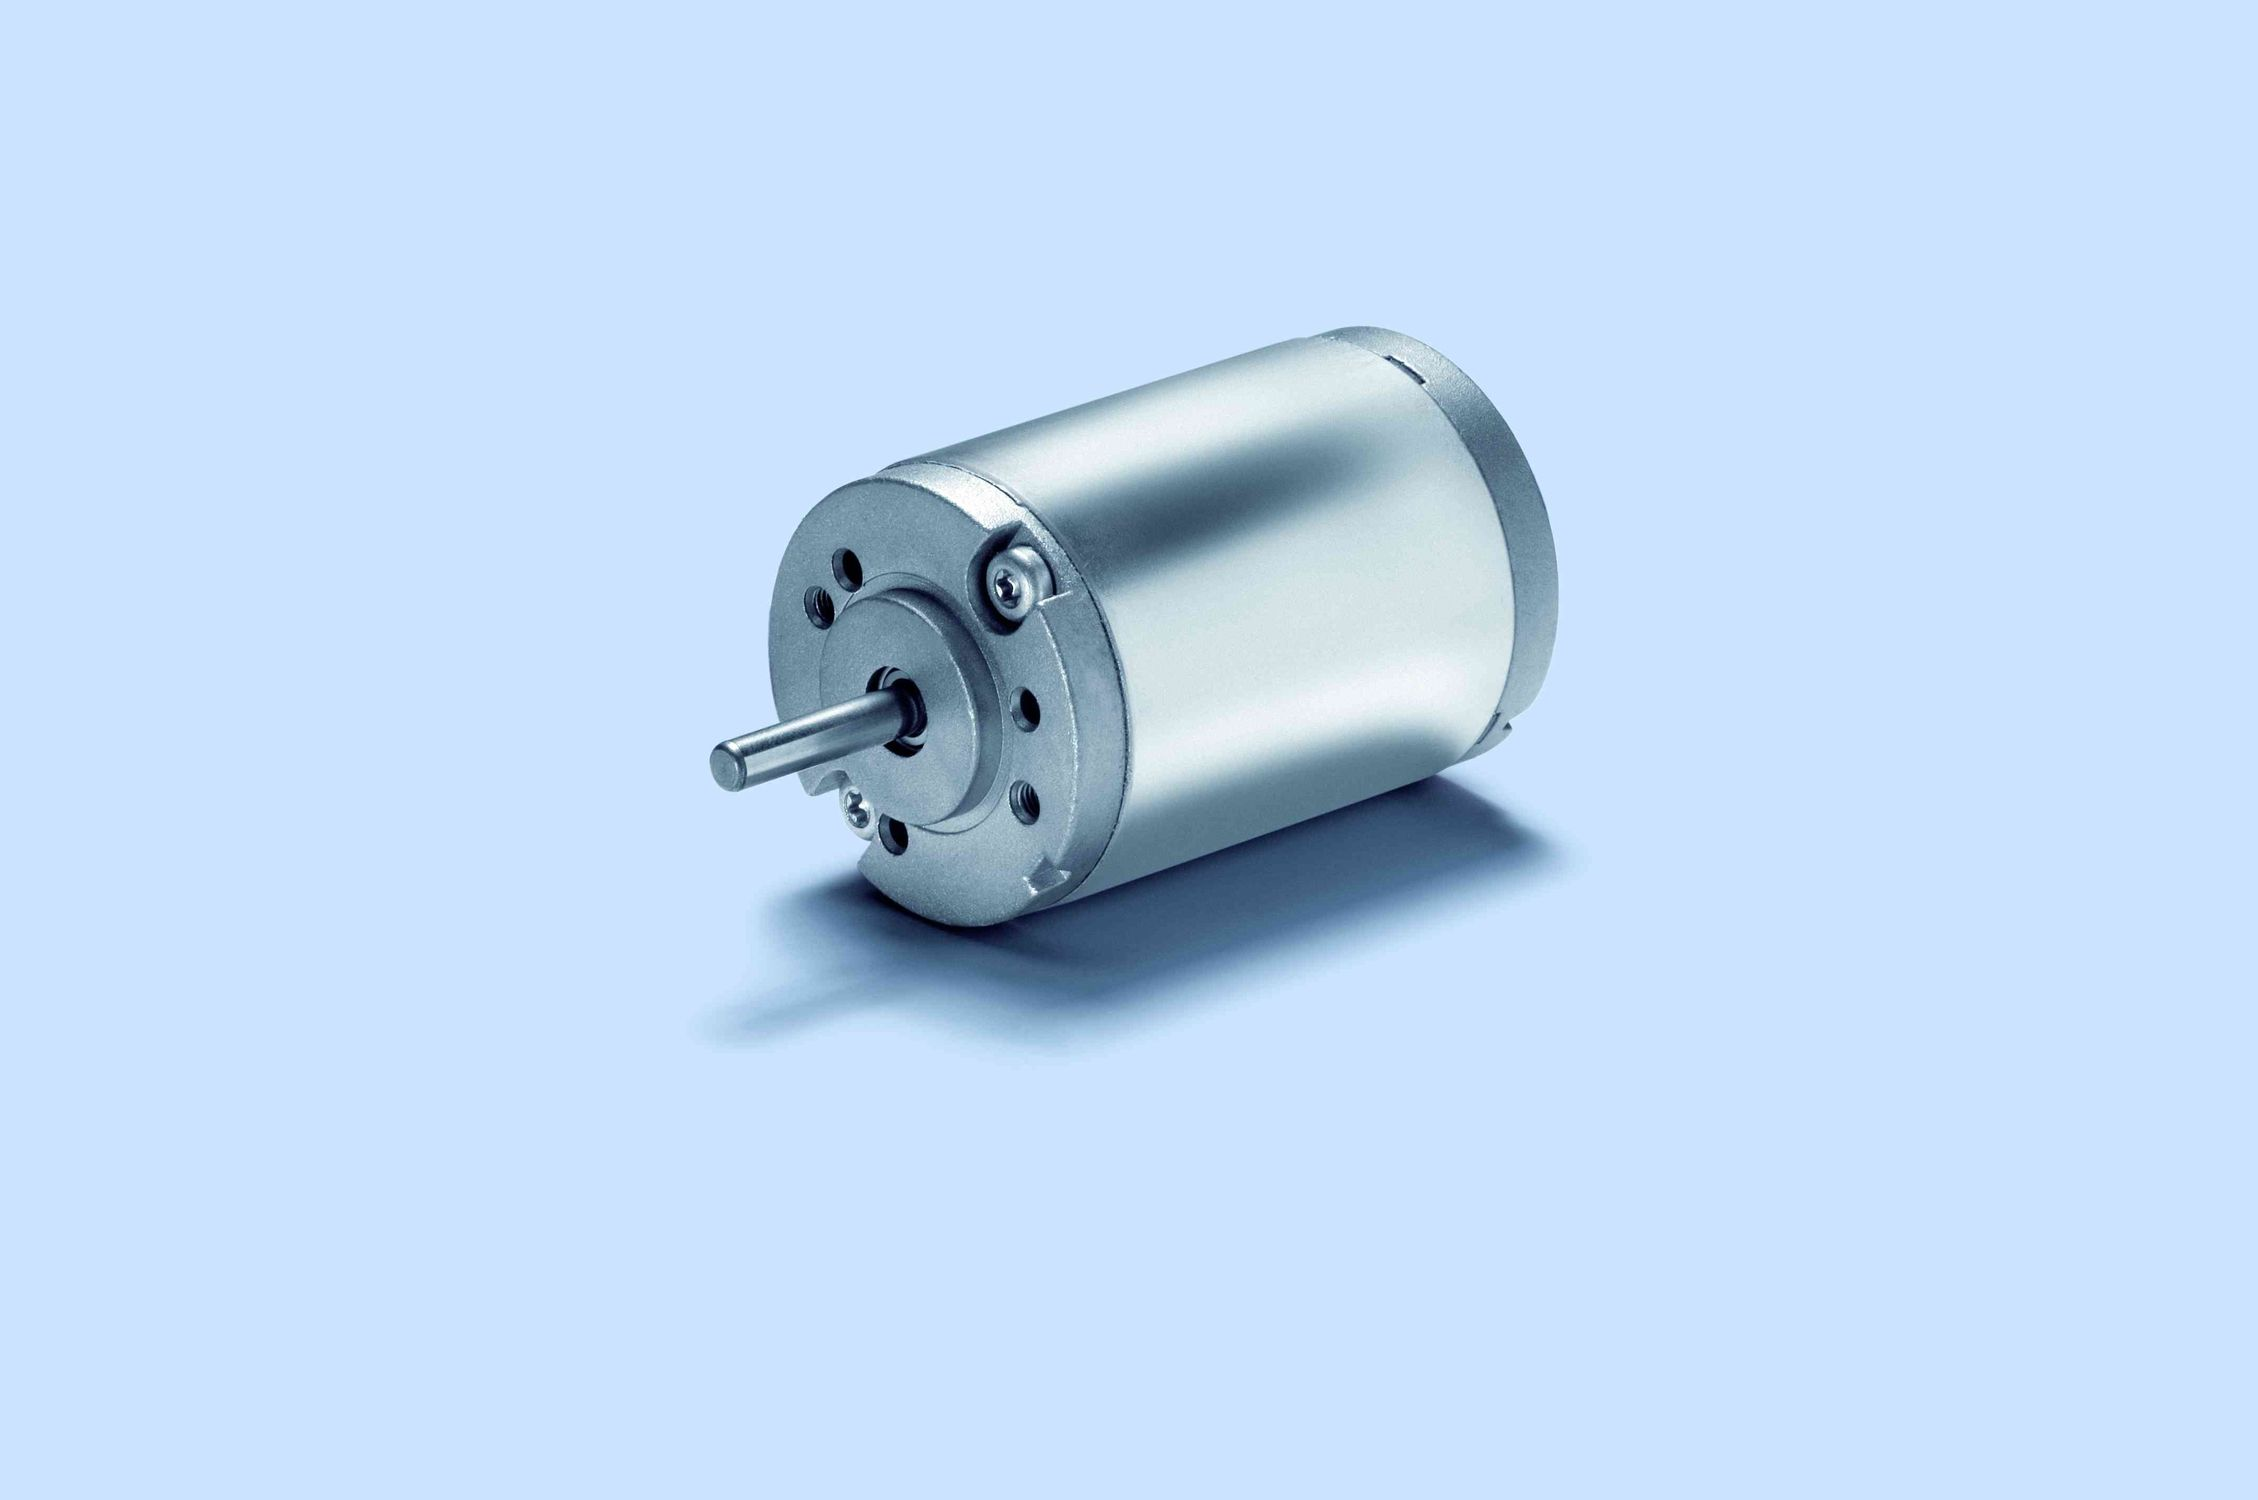
\includegraphics[width=0.4\textwidth]{Imatges/Funcionament/motor_continua.png}
			\caption{Motor de corriente continua}
			\label{fig:motor_continua}
		\end{figure}

El paso de corriente a través de las bobinas genera un campo magnético que reacciona con el campo magnético generado por los imanes, lo cual provoca un par de 	rotación y hace que el eje gire. Para mantener el giro indefinidamente, las bobinas 	están conectadas a una pieza llamada colector, de tal manera que van conmutando la 	polaridad al girar y se consigue crear un campo magnético pseudoestacionario.

			\begin{figure}
			\centering
			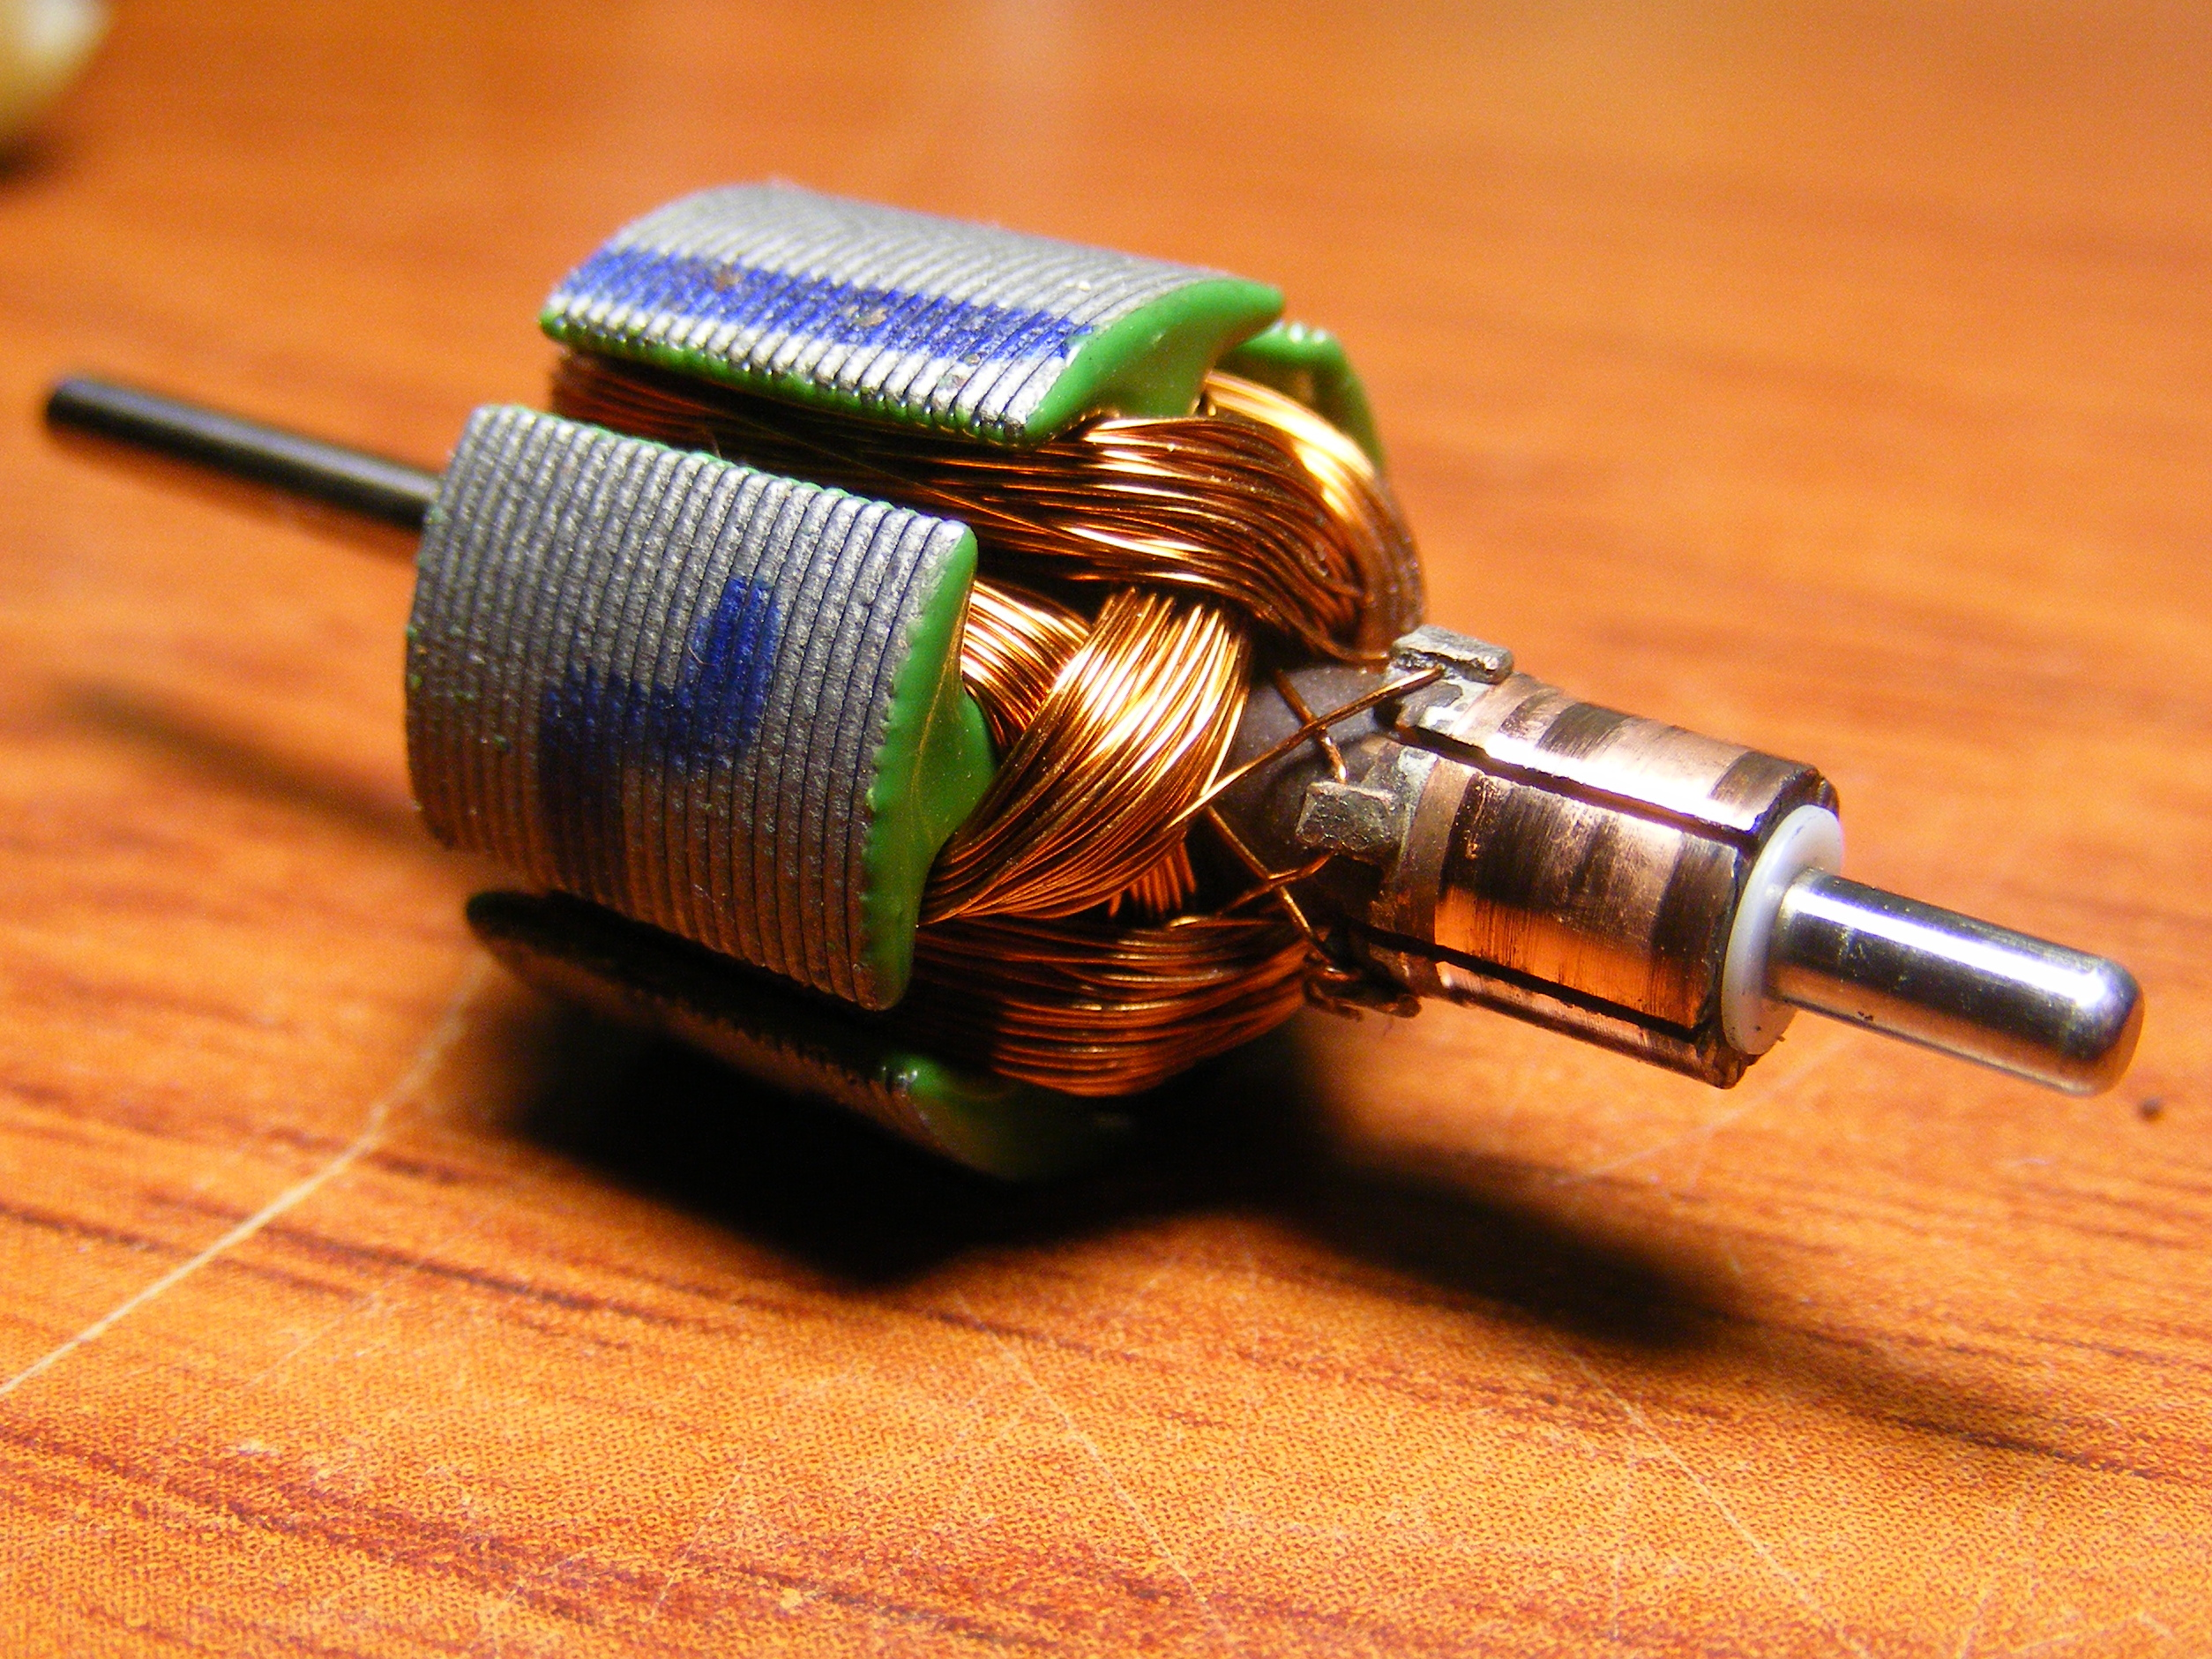
\includegraphics[width=0.4\textwidth]{Imatges/Funcionament/bobinas_motor_continua.png}
			\caption{Rotor de un motor de continua}
			\label{fig:bobinas_continua}
		\end{figure}
El gran defecto de estos motores es precisamente la presencia del colector de 	escobillas, ya que este sistema está sujeto a desgaste y es la causa principal de averías.

			\begin{figure}
			\centering
			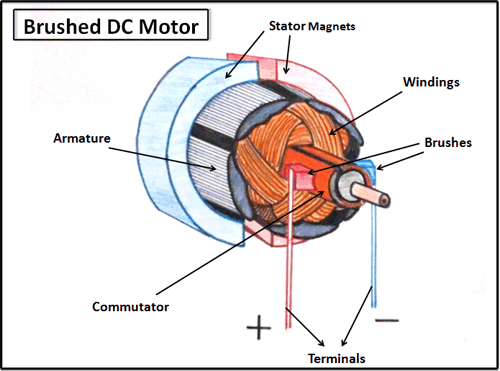
\includegraphics[width=0.5\textwidth]{Imatges/Funcionament/motor_continua_esquema.png}
			\caption{Esquema de un motor de continua}
			\label{fig:esquema_continua}
		\end{figure}

Como punto a favor, es el motor eléctrico más sencillo de controlar, ya que 	simplemente se controla aplicando una tensión continua en sus bornes. Como el flujo 	magnético del estator lo producen imanes permanentes, es constante, y la 	velocidad de rotación del motor se controla directamente mediante la ecuación $\omega_{m}=\frac{u_{r}}{\Phi_{r}}$; donde $\Phi_{r}$ es el flujo magnético del stator, $u_{r}$ la tensión aplicada y $\omega_{m}$ es la velocidad de rotación del motor.



	Muchas veces no es posible regular analógicamente la tensión de los bornes de 0V 	hasta la tensión nominal, ya que mediante electrónica digital esto no suele ser 	habitual. En esta situación se puede controlar el motor mediante técnicas PWM. Este 	sistema se basa en aplicar al motor unos ciclos de trabajo (duty cicles) que consisten en 	conectar y desconectar el motor a la tensión nominal, y se consigue el 	mismo 	efecto 	que con el control analógico por tensión.
	Dada una tensión de operación, el consumo de corriente por el motor es proporcional	a la cantidad de trabajo que está realizando. De esta manera, el consumo mínimo se 	produce cuando el motor gira en vacío (sin carga) y el máximo cuando el rotor se 	bloquea.

			\item Máquina brushless
			
			Su nombre viene de “Máquina de corriente continua sin escobillas”, en inglés 	brushless, aunque en realidad son motores trifásicos síncronos. Se los denomina de 	esta manera debido a que suelen llevar una electrónica que pasa de corriente continua 	a la trifásica que necesitan para funcionar, y de esta manera se controlan igual que los 	motores de continua.
			
	En su conFiguración más habitual o outrunner, se componen de un estator interno 	bobinado y un rotor externo con imanes permanentes, que es el que gira (Figura \ref{fig:motor_brushless}). También 	existen los inrunners, donde el rotor es interno.

			\begin{figure}
			\centering
			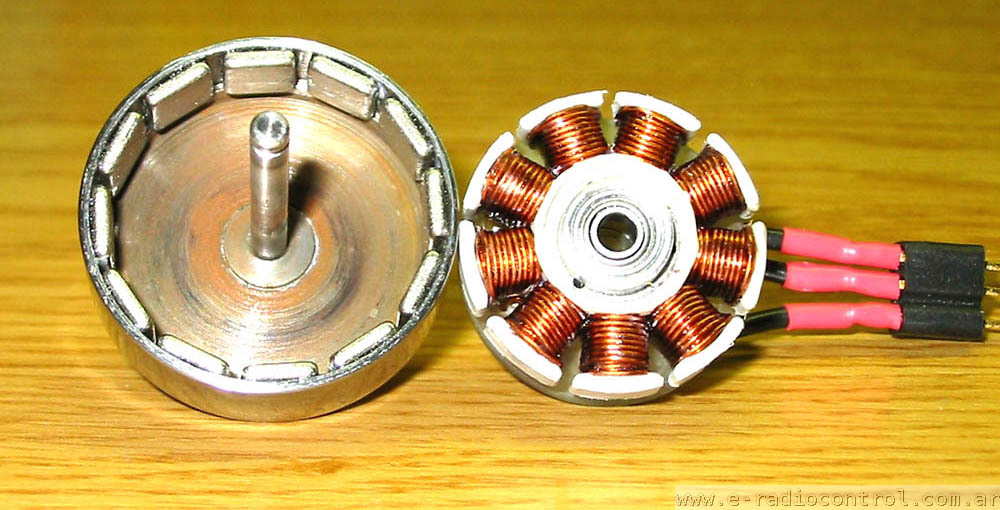
\includegraphics[width=0.5\textwidth]{Imatges/Funcionament/motor_brushless.png}
			\caption{Motor brushless (outrunner)}
			\label{fig:motor_brushless}
		\end{figure}
	
Mediante una electrónica que genera la corriente trifásica adecuada, se crea en el 	estator un campo magnético giratorio que arrastra los imanes del rotor. De esta 	manera, el rotor gira en sincronismo con el campo magnético generado (de aquí el 	nombre de máquina síncrona).

	Hoy en día, gracias al desarrollo de la electrónica, se muestran muy ventajosos, ya que 	son más baratos de fabricar, pesan menos para una misma potencia y requieren 	menos mantenimiento que los 	motores de continua con escobillas. Su único 	“problema” es que necesitan de una electrónica para funcionar, en el mundo del 	aeromodelismo conocida como ESC.
	
	Las características más relevantes a tener en cuenta son las siguientes:
		\begin{itemize}

			\item El voltaje nominal
			\item La velocidad de rotación nominal
			\item La corriente y potencia nominal
			\item Aspectos geométricos y peso
		\end{itemize}
	

		\end{itemize}
		
			\subsubsection{ESC (Variadores)}\label{subsubsec:ESC}
			
			Un ESC (Electronic Speed Controller) o variador, es un dispositivo electrónico que se encarga de controlar la velocidad de un motor eléctrico. En nuestro caso, los ESCs son variadores para motores brushless, es decir generan la corriente alterna trifásica de frecuencia variable que necesitan los motores para funcionar, a partir de la corriente continua de una batería (Figura \ref{fig:esc_conexiones}).
			
El ESC interpreta una señal de control, normalmente de tipo PWM, y asocia una cierta señal a una velocidad del motor (Figura \ref{fig:esc_pwm}). 
		\begin{figure}
			\centering
			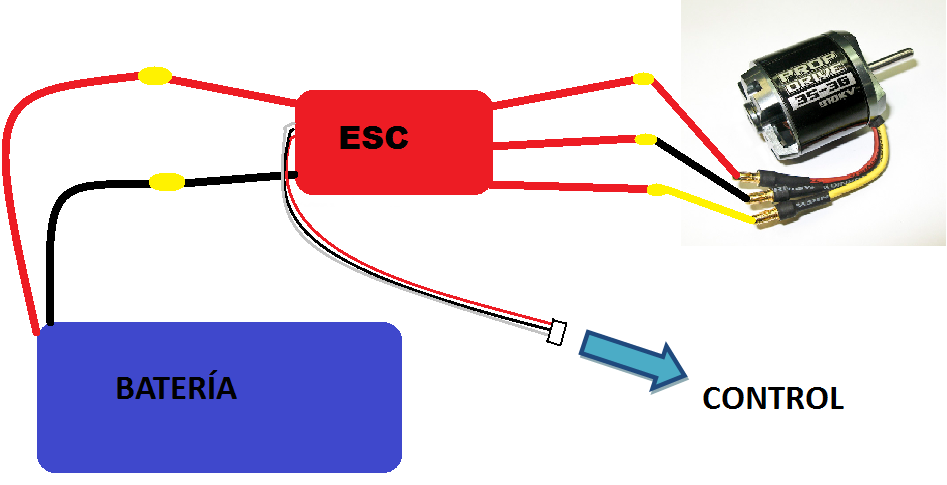
\includegraphics[width=0.8\textwidth]{Imatges/Funcionament/esc_conexiones.png}
			\caption{Esquema de conexiones del ESC}
			\label{fig:esc_conexiones}
		\end{figure}
		
		\begin{figure}
			\centering
			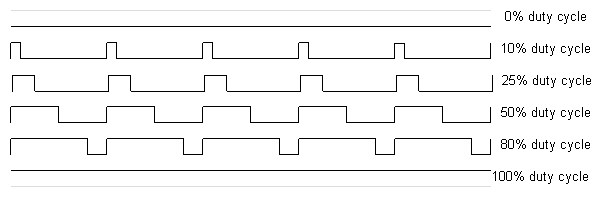
\includegraphics[width=0.8\textwidth]{Imatges/Funcionament/esc_pwm.png}
			\caption{Ejemplo de señal PWM}
			\label{fig:esc_pwm}
		\end{figure}

			

		Dependiendo de las características del motor hace falta un ESC adecuado. Para un tipo concreto de motor, el parámetro más relevante es el amperaje máximo del variador, el cual está relacionado con la potencia del motor que controla. También hay ESC’s programables en mayor o menor medida, pudiendo programar hasta curvas de aceleración.

			\begin{figure}
			\centering
			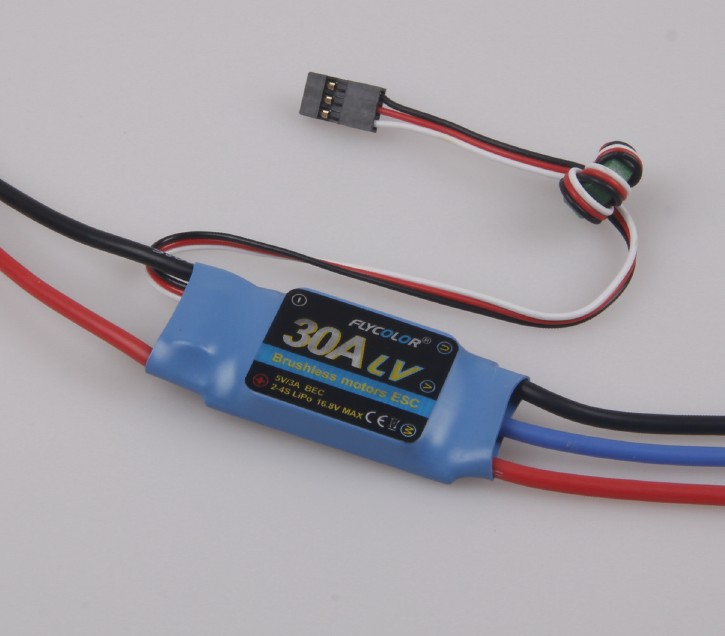
\includegraphics[width=0.8\textwidth]{Imatges/Funcionament/ESC.png}
			\caption{Imagen de un ESC real}
			\label{fig:ESC}
		\end{figure}

			
			\subsubsection{Hélices}\label{subsubsec:propellers}
			
			Las hélices son las responsables de obtener la sustentación necesaria a partir del giro de los motores. Cada aspa de la hélice se comporta igual que el ala de un avión, por este motivo las aspas tienen perfiles alares (Figura \ref{fig:Perfiles_alares}).
Un aspecto muy importante es la geometría de la hélice, que principalmente está determinada por los siguientes parámetros:
		\begin{itemize}
			\item Diámetro de la hélice
			\item Paso (Informa del ángulo de ataque del perfil, más paso es más ángulo de ataque)
			\item Tipo de perfil de las aspas (Figura \ref{fig:airfoil})
			\item Número de palas o aspas
		\end{itemize}
		
		\begin{figure}
			\centering
			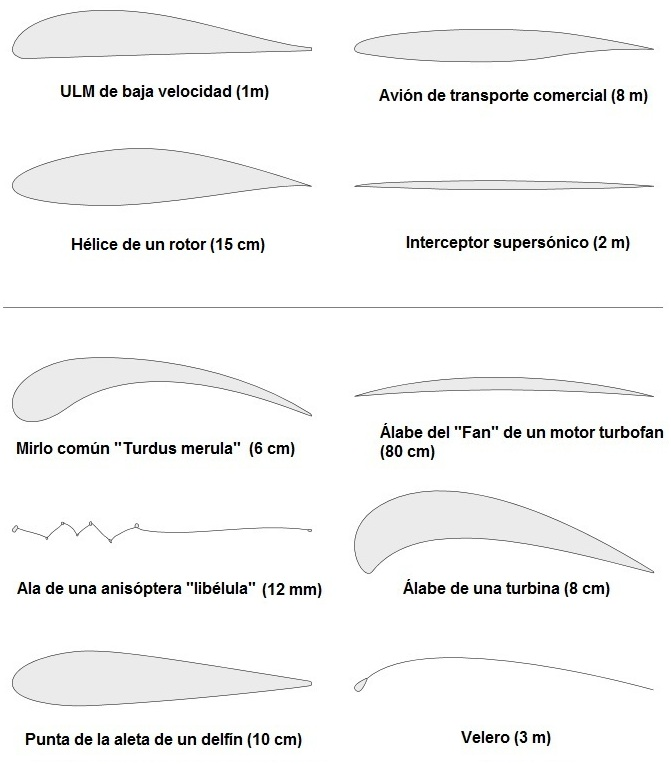
\includegraphics[width=0.7\textwidth]{Imatges/Funcionament/Perfiles_alares.png}
			\caption{Diferentes perfiles alares, tanto de la naturaleza como de distintos vehículos}
			\label{fig:Perfiles_alares}
		\end{figure}

		\begin{figure}
			\centering
			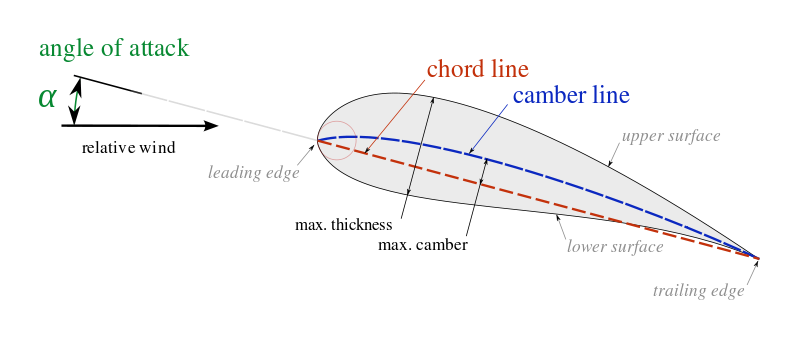
\includegraphics[width=0.7\textwidth]{Imatges/Funcionament/airfoil.png}
			\caption{Esquema de un perfil alar}
			\label{fig:airfoil}
		\end{figure}
		
		Una consideración a tener en cuenta es si la hélice es de paso fijo o de paso variable:
		\begin{itemize}
			\item De paso fijo: 
			
			Las palas son fijas al centro de la hélice, es decir, que la hélice es toda una sola pieza. Para conseguir más o menos sustentación se modifica la velocidad de rotación de la hélice.
			\item De paso variable: 
			
			Las palas pueden rotar sobre el centro de la hélice mediante un mecanismo adecuado, pudiendo variar su ángulo de ataque (Figura \ref{fig:paso_variable}). La sustentación depende de la velocidad de rotación y del paso, hay dos grados de libertad para controlarla.
		\end{itemize}

		En un cuadricóptero estas dos soluciones son totalmente factibles, pero presentan una serie de ventajas e inconvenientes:

		\begin{itemize}
			\item Paso fijo: 
			
			Muy económica, es la que más se utiliza con diferencia, tiene una gran facilidad de control (velocidad de rotación de los 4 motores independientes), es la más eficiente (no hay ningún mecanismo ni transmisión entre el motor y la hélice, ésta va fijada directamente al eje del motor) y tiene muy poco mantenimiento.
			
			\item Paso variable: 
			
			Cada rotor necesita un actuador (un servo) con un mecanismo complicado para variar el paso de cada hélice de manera independiente. Lo más utilizado es conectar mecánicamente los 4 rotores para que giren a la misma velocidad y controlar independientemente el paso de cada hélice. Permite hacer maniobras muy rápidas, pero es una solución más cara, requiere de más mantenimiento y es menos eficiente ya que hay elementos de transmisión entre el motor y la hélice.
			
			\begin{figure}
			\centering
			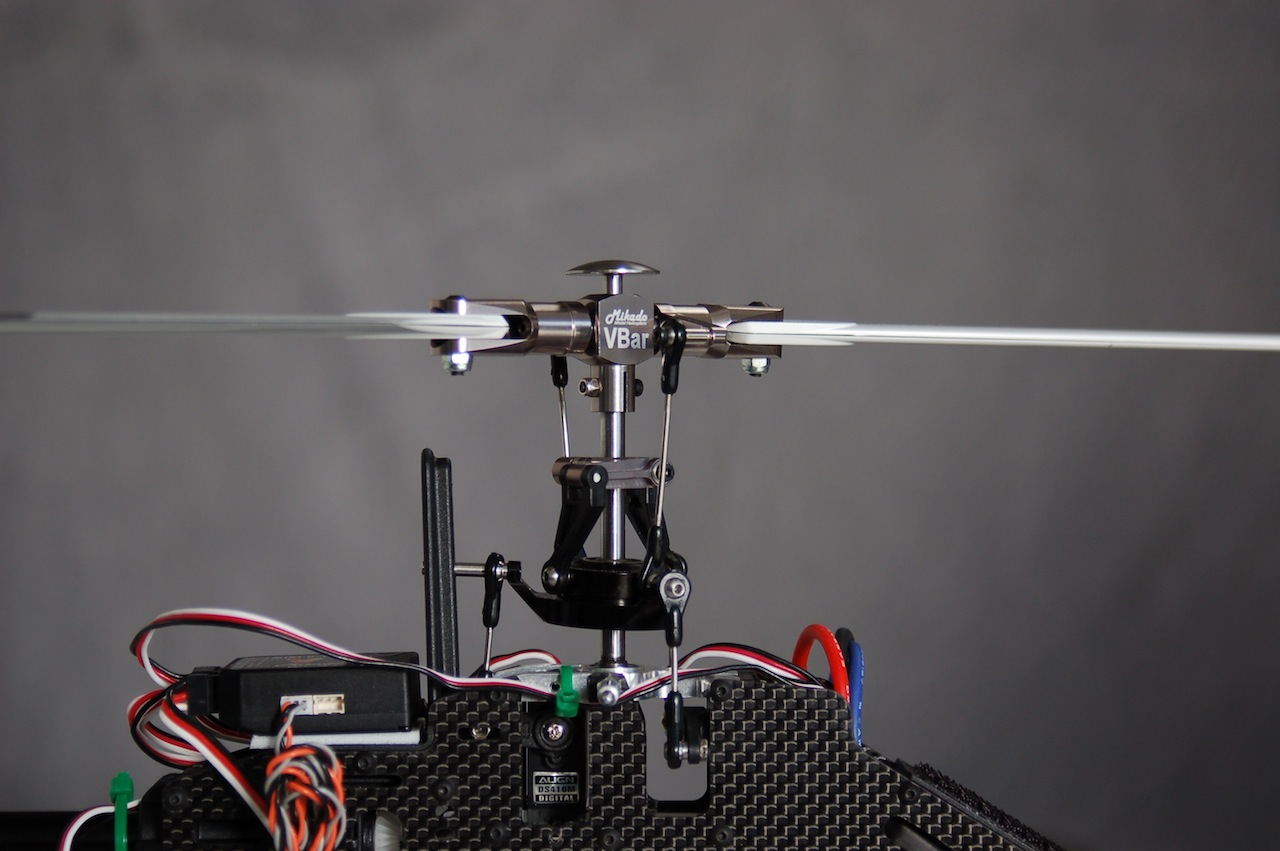
\includegraphics[width=0.7\textwidth]{Imatges/Funcionament/paso_variable.png}
			\caption{Imagen de una hélice con paso variable}
			\label{fig:paso_variable}
			\end{figure}
		\end{itemize}

		\subsection{Sistema de alimentación}\label{subsec:alimentacion}
		La energía eléctrica que necesita el cuadricóptero para funcionar se almacena en una o varias baterías, que en la mayoría de casos son recargables, permitiendo su utilización muchas veces. 
Proporcionan la energía al sistema de propulsión, pero también a los equipos electrónicos u otros accesorios que lleva el vehículo.
Se dividen en diferentes tipos, dependiendo de la tecnología que tienen para almacenar la energía. Entre los tipos más comunes utilizados hoy en día destacan: 

		\begin{itemize}
			\item Ni-CD (baterías de níquel-cadmio):

Existen desde hace mucho tiempo. Tienen efecto memoria, es decir, que pierden capacidad según el ciclo de carga-descarga que se les haga, no toleran bien las cargas rápidas y el cadmio que contienen es un material muy tóxico. Las hay de diferentes asociaciones de elementos, aunque destacan las de 7,2 voltios (una fila de 6 elementos o dos filas en serie paralelas de 3 elementos cada una).

			\item Ni-MH (baterías de níquel-metal-hidruro):

Surgieron al sustituir el cadmio por hidruros metálicos, haciendo que no sean tan contaminantes. Tienen el mismo voltaje por elemento y las más populares son las de 7,2 V. Tienen menos efecto memoria que las de Ni-CD, mayor capacidad y se pueden cargar rápido, pero aceptan un número menor de ciclos de carga. Tienen una resistencia interna elevada y no son adecuadas para suministrar potencias elevadas.

			\item Ion-Litio (baterías de iones de litio):

La capacidad de una batería de Ion-Litio es aproximadamente el doble de la capacidad de una batería de Ni-CD del mismo tamaño, gracias a que el litio es un metal poco pesado. El voltaje de una celda de Ion-Litio es de 3,7 voltios. No tienen mantenimiento y no poseen efecto memoria, por lo que no es necesario realizarles un reciclado cada cierto número de cargas, como en los dos tipos anteriores. Tienen una baja descarga durante su almacenamiento. Como desventaja, requieren de un circuito de control que se emplea para limitar el voltaje máximo de cada célula de la batería, para limitar el voltaje mínimo de descarga y también se hace un control de la temperatura para determinar cuando la batería está cargada. Un factor a tener en cuenta es que las baterías van perdiendo sus propiedades químicas con el tiempo, se haga o no uso de ellas. Para minimizar este efecto se recomienda almacenarlas con una carga del 40\% de su capacidad máxima en un lugar fresco, no exponerlas a altas temperaturas, no sobrecargarlas ni descargarlas en exceso. Si se descargasen por completo se podría invertir la polaridad con lo que no volverían a coger carga.
			\item Li-Po (baterías de polímero de litio):

Las baterías Li-Po son una variación de las de ión de litio, utilizan un polímero que les permite ser fabricadas en una mayor variedad de formas y tamaños que las de ión de litio. Tampoco tienen efecto memoria, y su mejor característica es que tienen una densidad de energía de entre 5 y 12 veces las de Ni-Cd o las de Ni-MH. El voltaje de cada celda es de 3,7 voltios. Además, tienen poca resistencia interna, por lo que su capacidad de descarga es elevada (se aprovecha casi el 100\% de la energía) y pueden alimentar dispositivos de mucha potencia. Como puntos en contra, tienen un voltaje mínimo de descarga más alto, si se descargan demasiado se pueden dañar e incluso explotar, y se deben cargar mediante cargadores especiales, siendo éstos más caros. Para almacenarlas se recomienda dejarlas a media carga. Con un uso adecuado, el tiempo de vida de estas baterías es superior al de las otras, aunque también se degradan con el tiempo. 
		\end{itemize}
		
De esta manera, las baterías de polímero de litio son las que presentan más ventajas, y están presentes a precios muy competitivos para prácticamente todas las aplicaciones, sobre todo en el campo del aeromodelismo.

Las características más importantes de una batería son:
		\begin{itemize}
			\item Tipo
			\item Voltaje (depende de la cantidad de elementos o celdas que tenga)
			\item Capacidad
			\item Máxima intensidad constante de descarga
			\item Máximo pico de intensidad de descarga (durante pocos segundos)
			\item Dimensiones y peso
		\end{itemize}


		\subsection{Sistema de control}\label{subsec:control}

			El cuadricóptero es un vehículo inestable que por sí solo no podría volar. Esto es debido a multitud de factores, por ejemplo a la imposibilidad de que los 4 rotores den exactamente el mismo empuje o a la acción de agentes externos como puede ser el viento. Por este motivo, el sistema necesita tener una realimentación (es decir, captar información de la realidad mediante sensores y compararla con las consignas deseadas) y actuar en consecuencia para mantener el vehículo estable en cualquier situación. 

Además, hace falta transformar la información de los 4 grados de libertad del control (acelerador, cabeceo, alabeo y guiñada) en la información que tiene que ir a cada uno de los 4 rotores. Los 4 grados de libertad de control pueden provenir de un sistema de control remoto manual, o de un sistema de navegación autónomo.

Juntando estos aspectos, el sistema de control de vuelo está formado por un sistema electrónico al que le llegan las señales de los 4 grados de libertad de control del vehículo, lee la información de múltiples sensores,  y actúa en consecuencia controlando los 4 rotores de manera independiente, permitiendo el vuelo estable de la aeronave.

Este sistema electrónico es habitualmente un microcontrolador con diferentes sensores y puertos de entrada/salida adecuados.

Entre los sensores más habituales están los sensores giroscópicos, los acelerómetros y los magnetómetros:
		\begin{itemize}
			\item Sensor giroscópico, o comúnmente llamado giroscopio o gyro en inglés: Detectan una aceleración angular en un eje (para saber si el vehículo cabecea, alabea o guiña)
			\item Acelerómetros: Detectan una aceleración en una dirección
			\item Magnetómetros: Detectan campos magnéticos (se utilizan principalmente como brújula para saber la orientación del vehículo)
		\end{itemize}
		Las placas más sencillas de control de vuelo pueden llevar solo 3 sensores giroscópicos en los 3 ejes ortogonales y un magnetómetro como brújula, pero placas más buenas pueden llevar hasta un giroscopio, un acelerómetro y un magnetómetro por cada eje, o incluso más sensores adicionales.

		\subsection{Sistema de navegación}\label{subsec:navegacion}

			Es el sistema encargado de guiar a la aeronave de manera autónoma. Puede estar integrado en el sistema de control de vuelo, o puede ser un sistema externo a éste. Hay diferentes tipos de navegación, como por ejemplo mediante GPS, con una navegación inercial (a partir de las aceleraciones detectadas en el vehículo)…

El sistema de navegación es el encargado de generar los 4 grados de libertad de control del vehículo que interpretará el sistema de control de vuelo, y de esta manera el vehículo puede desplazarse por una ruta determinada.


  \newpage
	\section{Diseño del cuadricóptero}\label{sec:diseno}


		\subsection{Diseño del chasis}\label{subsec:diseno_chasis}
Una vez decidida la conFiguración de cuadricóptero en X, es decir, que el eje de avance (x) está entre los rotores (Figura \ref{fig:conFiguracion_quad}), hizo falta estudiar qué solución estructural era más ventajosa. Los ejes del cuadricóptero que se han utilizado son el eje longitudinal “x”, el eje transversal “y” y el restante eje “z” que en el dibujo sale del papel. Las direcciones positivas corresponden a las del dibujo, es decir, el eje “x” hacia delante, el eje “y” hacia la izquierda y el eje “z” hacia arriba.

		\begin{figure}
			\centering
			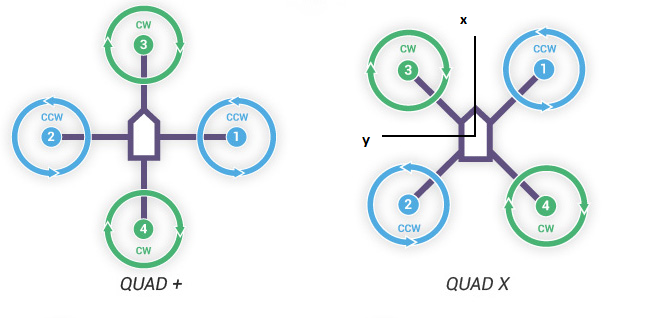
\includegraphics[width=0.7\textwidth]{Imatges/Disseny_Chasis/Quad_eixos.png}
			\caption{ConFiguración de los cuadricópteros}
			\label{fig:conFiguracion_quad}
		\end{figure}
		
Las posibles soluciones a considerar se agruparon en las siguientes familias:

		\begin{itemize}
			\item Forma de “H”: (Figura \ref{fig:chasis_H}) 

Se caracteriza por ser asimétrica entre los dos ejes “x” e “y”, por lo que estos dos momentos de inercia en principio no son iguales. Tiene una estructura principal más grande que compone el cuerpo del vehículo, y a ésta se le añaden las dos barras perpendiculares (que cada una puede estar a su vez formada por varias secciones) donde van los rotores.

		\begin{figure}
			\centering
			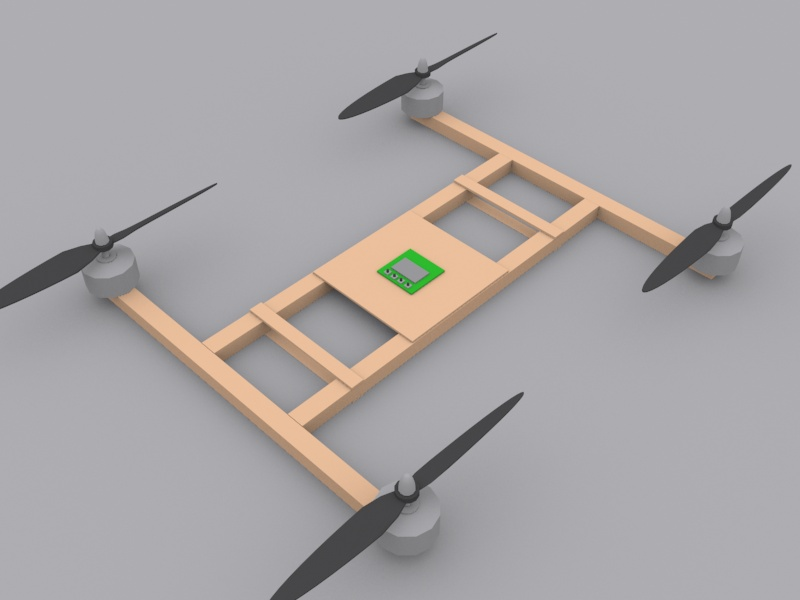
\includegraphics[width=0.7\textwidth]{Imatges/Disseny_Chasis/quadH.png}
			\caption{Chasis en forma de "H"}
			\label{fig:chasis_H}
		\end{figure}

Esta conFiguración permite tener mucho espacio disponible para alojar componentes en la parte central, y bien diseñada es muy robusta estructuralmente.
			
		\item Mediante una estructura de barras cruzadas en “X”:  (Figura \ref{fig:chasis_X})

Consistente en dos brazos superpuestos o cruzados por sus puntos medios y perpendiculares entre sí (también cada brazo puede estar formado por varios perfiles diferentes a su vez). En la parte central lleva la mayoría de componentes sobre unas estructuras de refuerzo. Tiene la ventaja de que es simétrica en los ejes “x” e “y”, aunque debido a que las barras se cruzan en la parte central no se optimiza el peso ni el espacio disponible.
		\begin{figure}
			\centering
			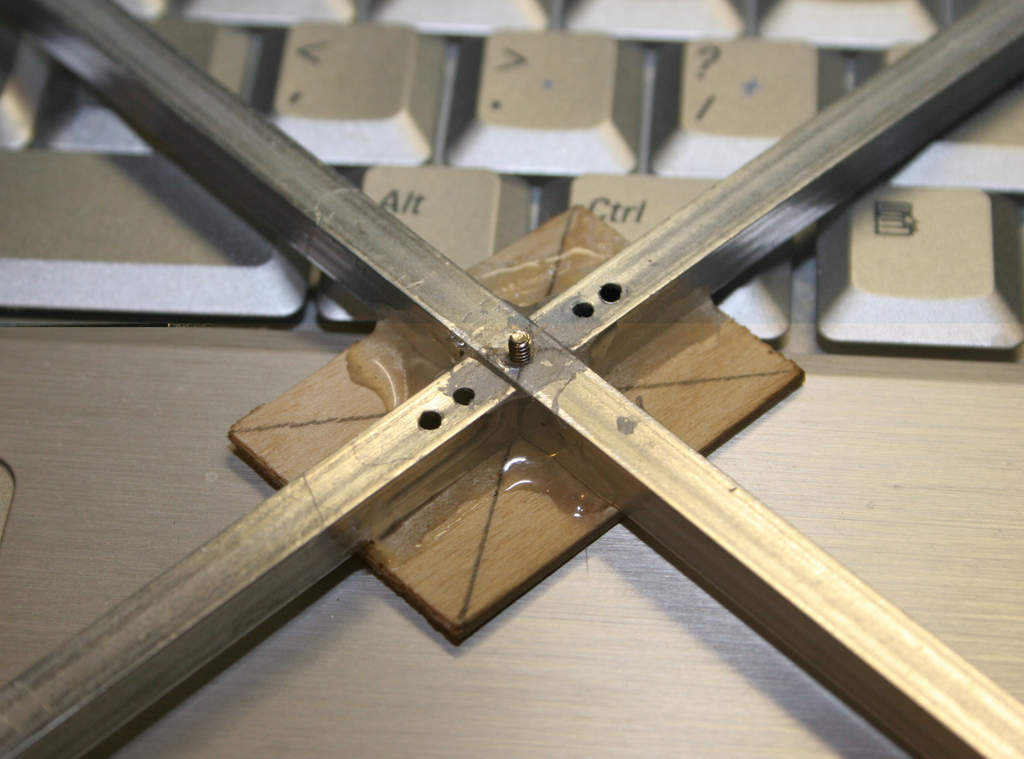
\includegraphics[width=0.7\textwidth]{Imatges/Disseny_Chasis/Chasis_barras_enteras.png}
			\caption{Estructura de barras cruzadas en "X"}
			\label{fig:chasis_X}
		\end{figure}

		\item Mediante barras en “X” unidas a una estructura central:  (Figura \ref{fig:chasis_X_central})

Esta solución consiste en una variación de la anterior, tiene 4 barras diferentes en vez de 2, sin continuidad en la parte central.
		\begin{figure}
			\centering
			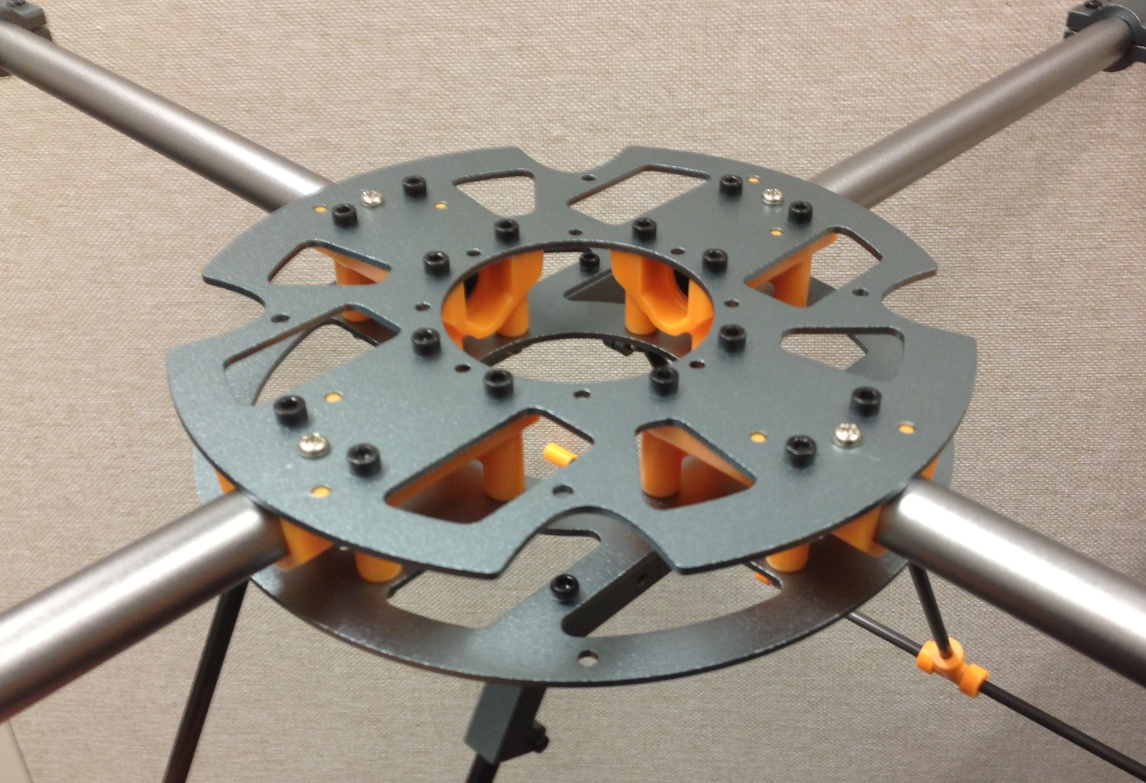
\includegraphics[width=0.7\textwidth]{Imatges/Disseny_Chasis/Chasis_4barras.png}
			\caption{Estructura de barras unidas a una estructura central}
			\label{fig:chasis_X_central}
		\end{figure}

De esta manera se puede aprovechar el espacio que queda en el centro para alojar algún componente a la vez que se elimina peso, ganando en modularidad (se puede desmontar un brazo sin afectar a los otros 3). Y la estructura central puede ser muy ligera sin afectar a una buena rigidez.
		\item En forma de cuadrado:  (Figura \ref{fig:chasis_cuadrado})

Se compone de una estructura que une los rotores entre ellos, en forma de cuadrado, y lleva algún tipo de soporte en la parte central para alojar el resto de componentes. También es simétrica en los ejes “x” e ”y” y es muy robusta.

		\begin{figure}
			\centering
			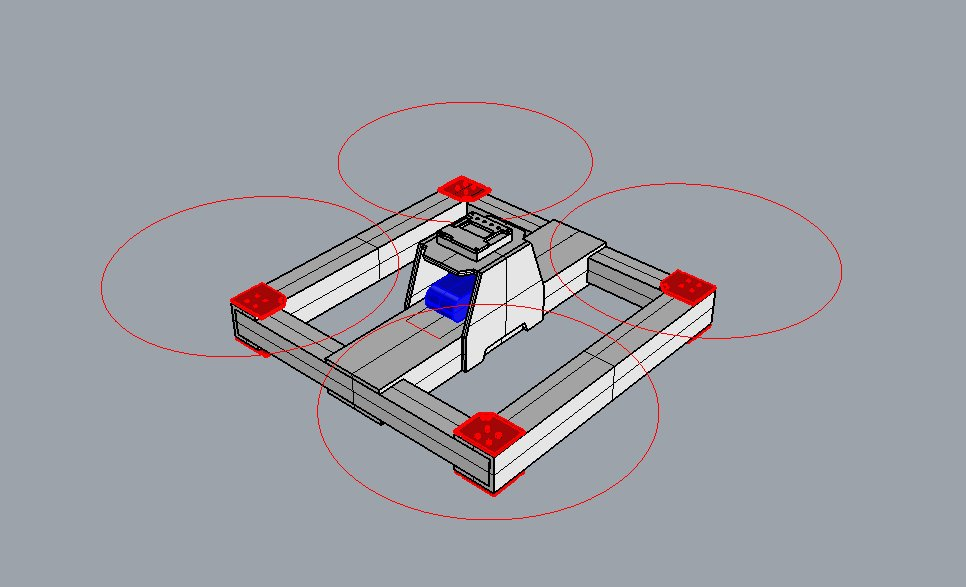
\includegraphics[width=0.7\textwidth]{Imatges/Disseny_Chasis/Chasis_cuadrado.png}
			\caption{Chasis cuadrado}
			\label{fig:chasis_cuadrado}
		\end{figure}
		\end{itemize}
		
Los criterios de diseño que se han utilizado se explican a continuación, en orden decreciente de prioridad: 
		\begin{itemize}
		\item Factor económico
		\item Minimizar la masa del conjunto (aumenta el tiempo de vuelo, la manejabilidad y la carga que se puede llevar encima)
		\item Facilidad de fabricación
		\item Buenas prestaciones estructurales (ante vibraciones, impactos, rigidez…)
		\item Modularidad del vehículo (para una fácil y rápida reparación o sustitución de componentes)
		\end{itemize}

		Teniendo en cuenta estos criterios, se ha elegido como óptimo una solución del tipo barras en “X” unidas a una estructura central, donde cada rotor va en la punta de una barra mediante una pieza de soporte del motor.

La dimensión principal del cuadricóptero (la distancia entre centros de los rotores) se ha elegido de 650 mm. Es una distancia un poco mayor que la mayoría de cuadricópteros existentes, que son de unos 450 o 550 mm, pero en ser un poco más grande vuela mejor y no hay problemas de espacio para componentes o accesorios que deba llevar, casi sin un aumento de peso del conjunto (Figura \ref{fig:dimensionado}).

		\begin{figure}
			\centering
			\includegraphics[width=1\textwidth]{Imatges/Disseny_Chasis/Croquis_chasis.png}
			\caption{Dimensionado básico de la estructura}
			\label{fig:dimensionado}
		\end{figure}

Las piezas de soporte de los motores se han adquirido ya hechas, son de fibra de vidrio y están pensadas para todo tipo de motores de tamaño similar a los nuestros. Cada una tiene una masa de 7,75 g, por lo que son muy ligeras (Figura \ref{fig:soporte_motor}).

El motor va anclado a su soporte mediante 4 tornillos de métrica 3. Se han elegido tornillos inoxidables con cabeza Allen M3x10 mm de rosca, para tener suficiente espacio para ponerle arandelas Grower y gomas entre el motor y el soporte para filtrar vibraciones. Las arandelas de apriete Grower son para que los tornillos no se aflojen con las vibraciones, y para más seguridad también se les ha puesto sellante de roscas.

La unión entre los soportes de los motores y las barras se hace mediante 2 tornillos M3 Allen con tuercas autoblocantes, para asegurar que no se aflojen con las vibraciones. Se ha observado, también, que poniendo un material que actúe como aislante entre el soporte y la barra se mejoran las vibraciones, como por ejemplo unas láminas de cartón.

		\begin{figure}
			\centering
			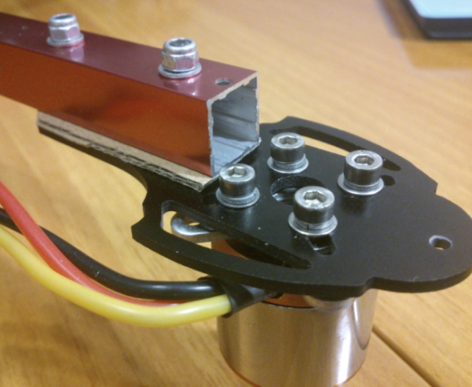
\includegraphics[width=0.6\textwidth]{Imatges/Disseny_Chasis/soporte_motor.png}
			\caption{Detalle del soporte del motor}
			\label{fig:soporte_motor}
		\end{figure}

Para las barras se han usado perfiles de aluminio. Con una sección adecuada, son casi igual de ligeros que perfiles de fibra de carbono pero mucho más baratos y con una buena rigidez estructural. Comparados con otros materiales como la madera, el plástico u otros metales, las propiedades del aluminio son superiores para esta pieza.

Se ha encontrado una sección cuadrada simétrica de 13x13 mm con paredes muy finas y 8 nervios internos. Cada barra de 250 mm de longitud tiene una masa de sólo 23 g. Además, al ser cuadrada se puede apoyar bien con otras superficies planas como los soportes de los motores o la estructura central (Figura \ref{fig:seccion_barras}).

		\begin{figure}
			\centering
			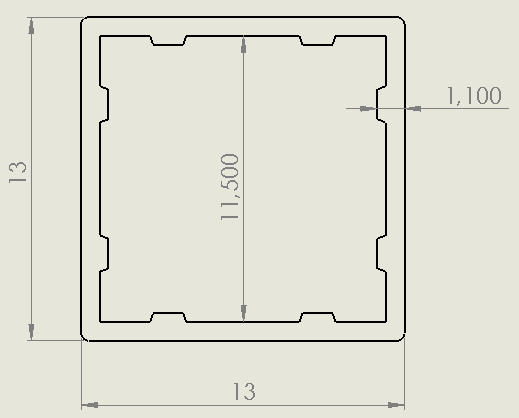
\includegraphics[width=0.6\textwidth]{Imatges/Disseny_Chasis/Seccion_barras.png}
			\caption{Sección de la barras de aluminio}
			\label{fig:seccion_barras}
		\end{figure}

Para la estructura central se tuvieron muchas ideas, pero la más sencilla e intuitiva resultó ser la mejor: Consiste en dos chapas cuadradas, una superior y otra inferior, que mediante tornillos aprietan las barras entre ellas. 

Como estas uniones son más críticas, se han utilizado tornillos M4 para mayor robustez. Con esta solución, es muy fácil desmontar un brazo entero de la estructura si es necesario sin afectar al conjunto. También se pueden aprovechar los finales de rosca de los tornillos para sujetar ciertas cosas, como se ve más adelante.

La elección del material para estas piezas seleccionó a la madera de contrachapado como óptima, siendo la solución adoptada madera de contrachapado de 3,5 mm de espesor. Es un material muy barato y muy fácil de fabricar, siendo además de los más ligeros. Cualquier chapa de aluminio es demasiado cara y más pesada, y de manera análoga pasa con los plásticos. La madera, además, absorbe vibraciones y tiene buenas propiedades mecánicas, y el contrachapado tiene la ventaja que no tiene dirección de fibras, con lo cual es bastante isotrópico.

		\begin{figure}
			\centering
			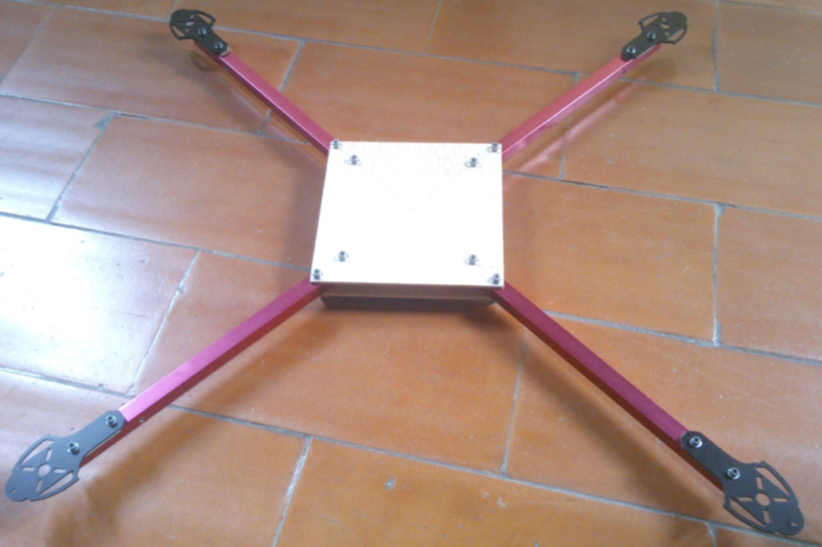
\includegraphics[width=0.8\textwidth]{Imatges/Disseny_Chasis/quad_frame.png}
			\caption{Conjunto del chasis con los soportes de los motores}
			\label{fig:quad_frame}
		\end{figure}

El peso del conjunto del chasis con los soportes de los motores es de 243 g (Figura \ref{fig:quad_frame}).
En el espacio entre las dos chapas centrales va alojado el sistema de distribución eléctrico de los motores, es decir, de la batería a cada uno de los 4 variadores, y éstos van cogidos a los 4 lados. De esta manera, la mayoría de los cables quedan escondidos dentro de la estructura, quedando protegidos y dejando totalmente libres las superficies superior e inferior del chasis (Figura \ref{fig:conexiones_esc}).

		\begin{figure}
			\centering
			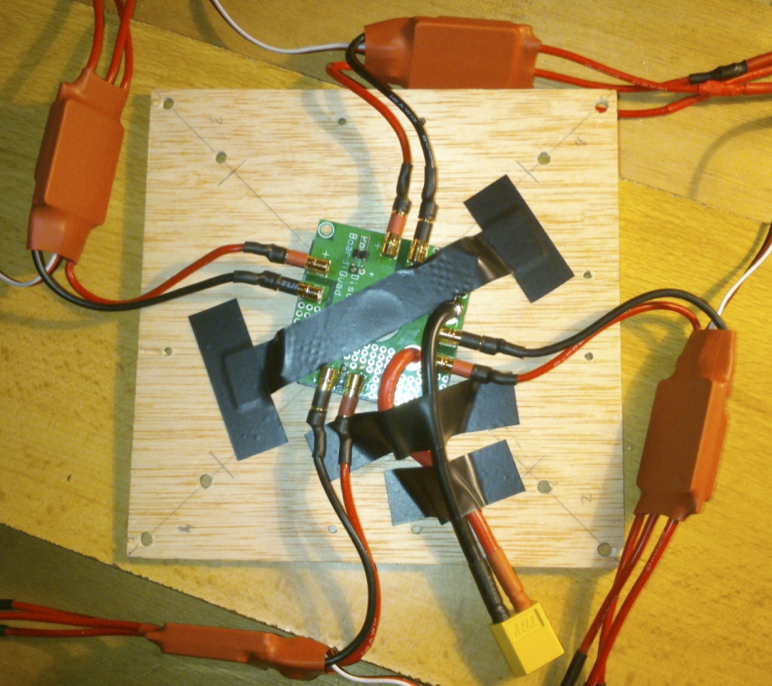
\includegraphics[width=0.7\textwidth]{Imatges/Disseny_Chasis/conexiones_esc.png}
			\caption{Sistema de distibución eléctrico de los motores}
			\label{fig:conexiones_esc}
		\end{figure}

En la superficie superior hacia arriba se dispone la electrónica, y en la inferior hacia abajo la batería, para disminuir el centro de gravedad respecto al plano de las hélices y ganar estabilidad.


		\subsection{Diseño del tren de aterrizaje con suspensión}\label{subsec:diseno_suspension}
En todas las aeronaves, el aterrizaje es seguramente la maniobra más delicada y peligrosa. Y es por este motivo que es de vital importancia diseñar un buen sistema que garantice la integridad y la seguridad de las tomas de tierra. 

\newpage
\maketitle

	\section{Elección de los componentes del cuadricóptero}\label{sec:componentes}
	
	Una vez elegido el tamaño aproximado del cuadricóptero (650mm entre ejes, sección \ref{subsec:diseno_chasis}) se tuvieron que escoger los componentes adecuados (descritos anteriormente en la sección \ref{sec:funcionamiento}) para hacerlo funcionar. 
	
		\subsection{Elección del sistema de propulsión y alimentación}\label{subsec:componentes_prop_alim}
			
			La elección del sistema de propulsión va entrelazada con la del sistema de alimentación, y los dos sistemas, a su vez, dependen del factor más importante en el cuadricóptero: el peso. Cuanto más peso tenga el cuadricóptero, más potencia necesitará de los motores y de las hélices, y éstos necesitarán que la batería sea suficiente para abastecerlos. Por este motivo, se ha estimado el peso que podría tener nuestro cuadricóptero y a partir de ahí se han escogido los componentes de propulsión y alimentación. Cada uno de los componentes tiene sus características propias, que lo definen para una u otra utilidad:
	
	\begin{itemize}
		
		\item Motor
		
		El motor es un elemento determinante del cuadricóptero, y tiene que ser elegido correctamente para un buen funcionamiento. Las especificaciones más relevantes para escoger un motor son:
			
			\begin{itemize}
				\item Voltaje que soporta [$V$]: 
				
				Normalmente está indicado en función de las celdas en serie de una batería de polímero de litio (Li-Po). Por ejemplo, un motor que soporte voltajes de 2S (dos celdas en serie de una Li-Po) hasta 4S significa que puede trabajar con voltajes de $3,7\times 2=7,4V$ hasta $3,7\times 4=14,8V$. Es importante tener en cuenta este voltaje a la hora de elegir la batería y los variadores para evitar sobrecalentamientos y un mal funcionamiento del conjunto.
				
				\item Constante de velocidad del motor $K_{v}$: 
				
				Se mide en $(min\times V)^{-1}$, es decir, en revoluciones por minuto por cada Volt, normalmente indicado como $rpm/V$. La constante indica la velocidad angular (en $min^{-1})$ del motor en función del voltaje ($V$) de entrada, en un caso ideal del motor sin carga externa. Esta constante del motor y el voltaje al cual se somete son determinantes para la elección de la hélice, ya que habrá que elegirla de forma que haga trabajar el motor en unos régimenes correctos y el máximo eficientes posibles.
				
				\item Potencia del motor [$W$]:
				
				Indica la potencia máxima que podrá ofrecer el motor. La potencia que pueda ofrecer el motor dependerá totalmente de las hélices. Como la potencia es el producto del voltaje por la intensidad ($W=V\times I$), hay que mirar qué potencia da el motor en este caso, ya que el fabricante normalmente mostrará la potencia máxima que da el motor con el voltaje e intensidad máximas.
				
				\item Intensidad máxima del motor [$A$]:
				
				Indica la intensidad máxima a la que el motor funciona correctamente. Es preferible que el motor no se acerque a este valor para evitar el sobrecalentamiento.
				
				\item Resistencia interna [$\Omega$]:
					
				Característica relevante para conocer la eficiencia del motor. Cuanta más alta sea esta resistencia interna, más altas serán las pérdidas por efecto Joule del motor y peor será su rendimiento.
				
				\item Otras especificaciones, como el tamaño, el peso y aspectos geométricos.
			\end{itemize}
			
		\item Hélices
		
		Las hélices son unos elementos clave para el cuadricóptero. De ellas depende la sustentación y tienen que estar bien dimensionadas para levantar el peso del aparato sin que ésto suponga demasiado esfuerzo para los motores. Las especificaciones más relevantes para escoger las hélices son:
		
		\begin{itemize}
			\item Diámetro de la hélice [$inch$]:
			
				El diámetro de la hélice, normalmente indicado comercialmente en pulgadas, es una especificación básica a la hora de elegir. Cuanto más grande sea la hélice, más resistencia ofrece al motor y por lo tanto gira más lento. Esta reducción de velocidad resulta beneficiosa ya que las pérdidas aerodinámicas por fricción son menores. El diámetro también influye en el comportamiento del cuadricóptero: Cuanto más pequeñas sean el comportamiento será más brusco y rápido; cuanto más grandes el comportamiento será más lento y estable.
				
			\item Paso de la hélice [$inch$]:
			
				El paso de la hélice se indica comercialmente en pulgadas de avance por cada vuelta dada. Esta característica indica la velocidad de avance de la hélice: cuanto más grande sea, más rápido se empuja el aire y más fuerza tiene que hacer el motor. En los cuadricópteros es mejor tener un paso pequeño, ya que es preferible tener más fuerza de sustentación para levantar el peso que velocidad.
				
			\item Número de aspas:
			
				Cuantas más aspas tenga una hélice, más volumen moverá a menos revoluciones. Aun así, el rendimiento baja si se añaden más aspas. Normalmente las hélices de los cuadricópteros tienen 2 aspas, las mínimas, para ser más eficientes y tener más autonomía.
				
			\item  Tipo de perfil de las aspas, bastante estándard.
				
		\end{itemize}
		
		\item Variadores (ESC)
		
		Los ESC controlan la velocidad de los motores, y por lo tanto tienen que poder soportar el voltaje y la intensidad de éstos. Por eso, hay que elegir variadores del mismo voltaje que la batería y el motor, y preferiblemente con un buen margen de una intensidad máxima soportada respecto a la intensidad máxima del motor, para evitar problemas con los picos de corriente. También se pueden elegir programables en mayor o menor medida, dependiendo de las necesidades.
		
		Muchos ESC también incorporan un BEC (Battery Eliminator Circuit), un circuito electrónico destinado a alimentar a 5V toda la electrónica de control, evitando así una batería dedicada a eso.
		
		\item Batería
		
		La batería es probablemente el componente más pesado del cuadricóptero, y por lo tanto hay que elegirla correctamente para tener una buena relación entre peso y autonomía. Las usadas en aeromodelismo normalmente son las de polímero de litio (Li-Po), por esa razón sólo se hace referencia a baterías de este tipo. Una batería Li-Po comercial tiene las siguientes características:
			
		\begin{itemize}
			\item Distribución de celdas
			
			Las baterías tienen un código para indicar como están distribuidas las celdas. Se indica con un número seguido de una ``S'', que indica el número de celdas en serie que tiene la batería, y que por lo tanto indica el voltaje de ésta; y de otro número seguido por una ``P'', que indica el número de celdas en paralelo, que no influyen en el voltaje (a veces no se indica) pero sí en la capacidad.
			
			Por ejemplo, una batería ``3S1P'' es una batería de sólo 3 celdas en serie, con un voltaje de $3,7V\times 3=11,1V$.
			
			\item Capacidad [$mAh$]
			
			Es un parámetro clave para saber la energía que puede acumular. Se mide en $mAh$ y sólo hace falta multiplicar el valor por el voltaje de la batería para tener una unidad de energía [$mW\times h$].
			
			Por ejemplo, si tenemos una batería de 3S de $5000mAh$, podemos tener una corriente de $5A$ durante una hora, $10A$ durante media hora, etc\ldots Su energía acumulada es, entonces: $3,7\times 3=11,1V\times 5Ah=55,5Wh$.
			
			\item Máxima intensidad constante de descarga [``C'']
			
			La máxima intensidad de descarga se mide en ``C'', que significa el número de veces que puede descargar su propia capacidad en Amperios. Por ejemplo, para la batería anterior de 3S 5000mAh, si su máxima capacidad de descarga es 20C, significa que su máxima intensidad que puede dar son: $20\times 5A= 100A$. A veces también se indica el máximo pico de intensidad de descarga durante unos segundos, también en ``C''.

			\item Dimensiones y peso
			
			El peso de la batería es un factor a tener muy en cuenta a la hora de elegir. Cuanta más capacidad tenga la batería, más peso tendrá, así que hay que estudiar la autonomía total del cuadricóptero en función del peso extra que supone añadir baterías de más capacidad.
			
		\end{itemize}
	\end{itemize}
	
	
	Para escoger estos componentes, y en función del tamaño del cuadricóptero, se ha hecho una estimación del peso total de $1,5Kg$ incluyendo una batería de bastante capacidad. A partir de aquí, se han estudiado combinaciones de componentes para poder levantar este peso.
	
	\subsubsection{Criterios de elección}\label{subsubsec:criterios}
	
		Los criterios para seleccionar los componentes han sido los siguientes:
		
		\begin{itemize}
			\item Máxima autonomía y eficiencia:
					
					\begin{itemize}
						\item Batería de mucha capacidad
						\item Hélices eficientes: de dos aspas, de diámetro grande y de paso pequeño
						\item Motores eficientes con poca resistencia interna
					\end{itemize}
			\item Potencia suficiente para levantar futuros accesorios
				
				\begin{itemize}
					\item Motores potentes: Que puedan levantar el doble de peso del propio cuadricóptero
					\item Motores que puedan mover hélices grandes: Motores con una $K_{v}$ pequeña, para tener más fuerza con poca velocidad 
				\end{itemize}
			\item Componentes de buena calidad y económicos
		\end{itemize}
	
	\subsubsection{Elección de los componentes}\label{subsubsec:eleccion}
			
			\begin{itemize}
			
				\item Batería:
				
				El voltaje de la batería para alimentar los motores está entre las 2S (7,4V) y las 4S (14,8V). Una batería de 2S tendría que entregar mucha intensidad para poder lograr la potencia necesaria para levantar el cuadricóptero, así que se descarta. En el otro extremo, la batería de 4S puede entregar mucha potencia, pero al tener un voltaje elevado se necesitarían motores muy lentos para tener una buena eficiencia (sección \ref{subsubsec:criterios}). Motores con una $K_{v}$ tan reducida acostumbran a ser bastante más caros, así que se ha optado por una batería de tres celdas 3S, con una capacidad elevada de 5000mAh y 20C (100A de descarga continua) (Figura \ref{fig:bateria_nuestra}).
								
			\begin{figure}
					\centering
					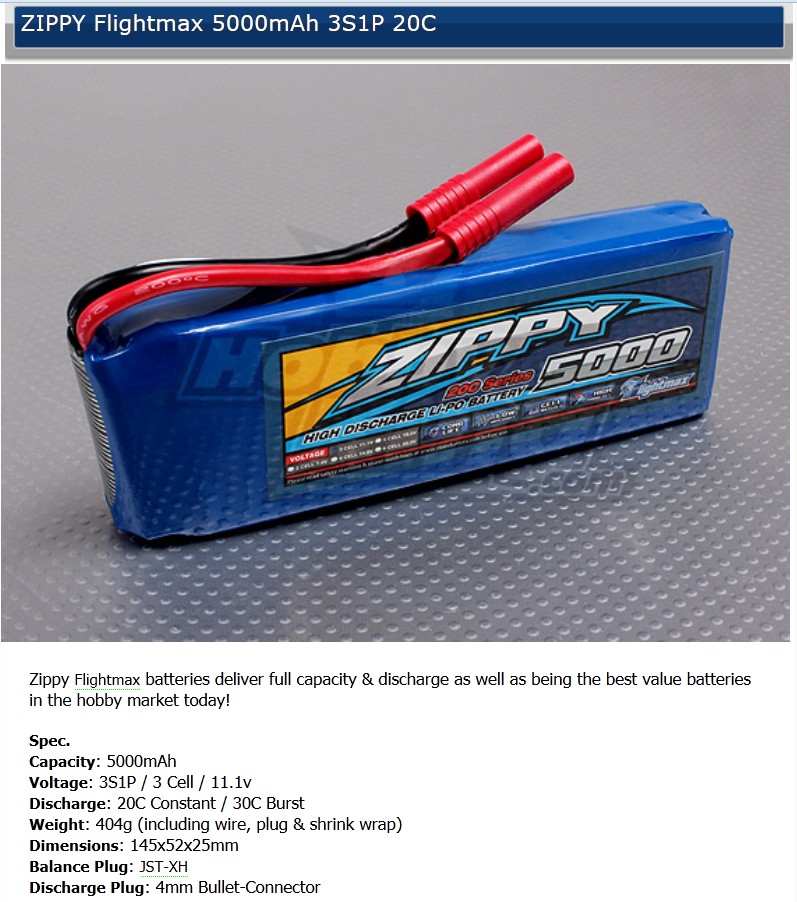
\includegraphics[width=0.8\textwidth]{Imatges/Componentes/bateria.png}
					\caption{Bateria escogida}
					\label{fig:bateria_nuestra}
			\end{figure}
									
				\item Motores:
				
				Como ya se ha comentado en el apartado anterior (\ref{subsubsec:criterios}), se requieren unos motores potentes con una $K_{v}$ reducida que funcionen bien con $11,1V$, que sean robustos, eficientes y de buena calidad, además de económicos. Después de un estudio entre numerosos motores de bajo coste (hay que comprar cuatro), se han elegido los de la Figura \ref{fig:motor_nuestro}.
				
				\begin{figure}
					\centering
					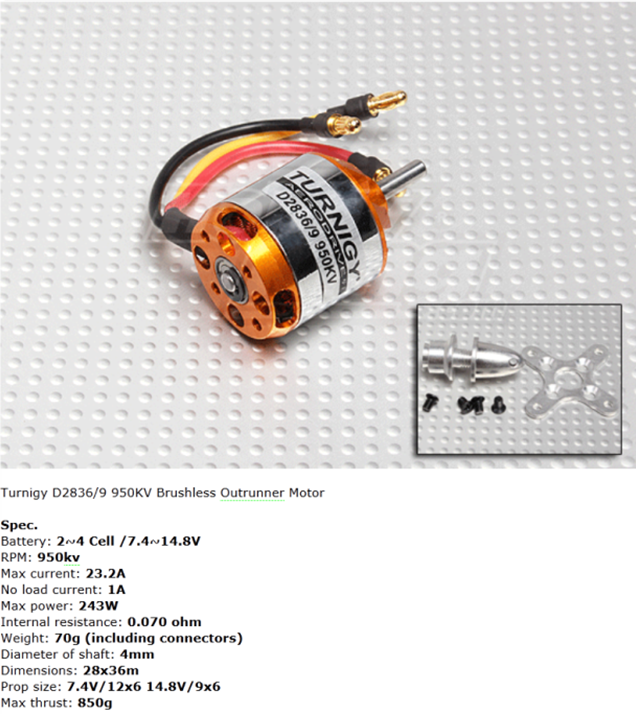
\includegraphics[width=0.8\textwidth]{Imatges/Componentes/motor.png}
					\caption{Motor escogido}
					\label{fig:motor_nuestro}
				\end{figure}
				
				\item Hélices:
				
				Para elegir el tamaño correcto de las hélices se ha hecho un estudio de comportamiento con una potente herramienta de Internet. El motor elegido funciona con hélices de tamaño desde 8 pulgadas hasta 12 pulgadas. Por esta razón, se han puesto en una calculadora los parámetros del motor escogido y diferentes tipos de hélices para decidir:
				
				\begin{itemize}
					\item 8x4,5 (Figura \ref{fig:8inch})
							\begin{figure}
								\centering
								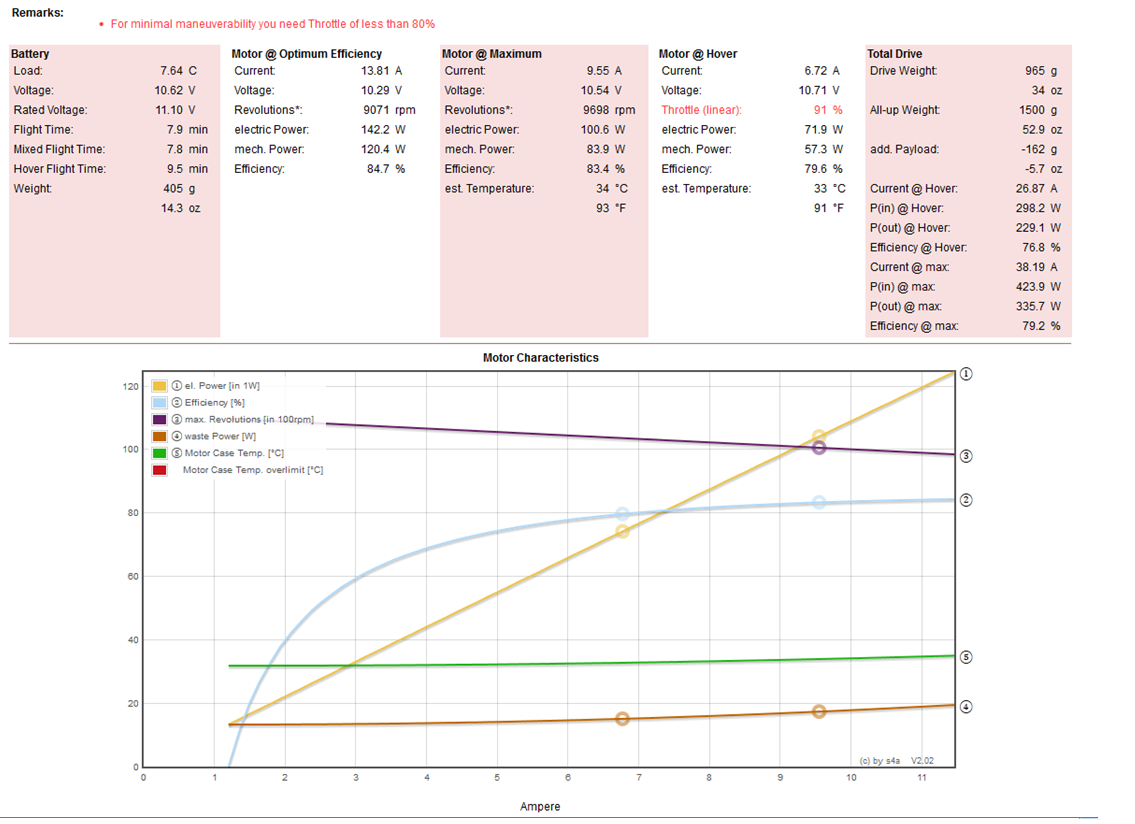
\includegraphics[width=1\textwidth]{Imatges/Componentes/8x4_5.png}
								\caption{Estudio con hélices de 8 pulgadas de diámetro y 4,5 pulgadas de paso}
								\label{fig:8inch}
							\end{figure}
							
					\item 10x4,5 (Figura \ref{fig:10inch})
					\begin{figure}
								\centering
								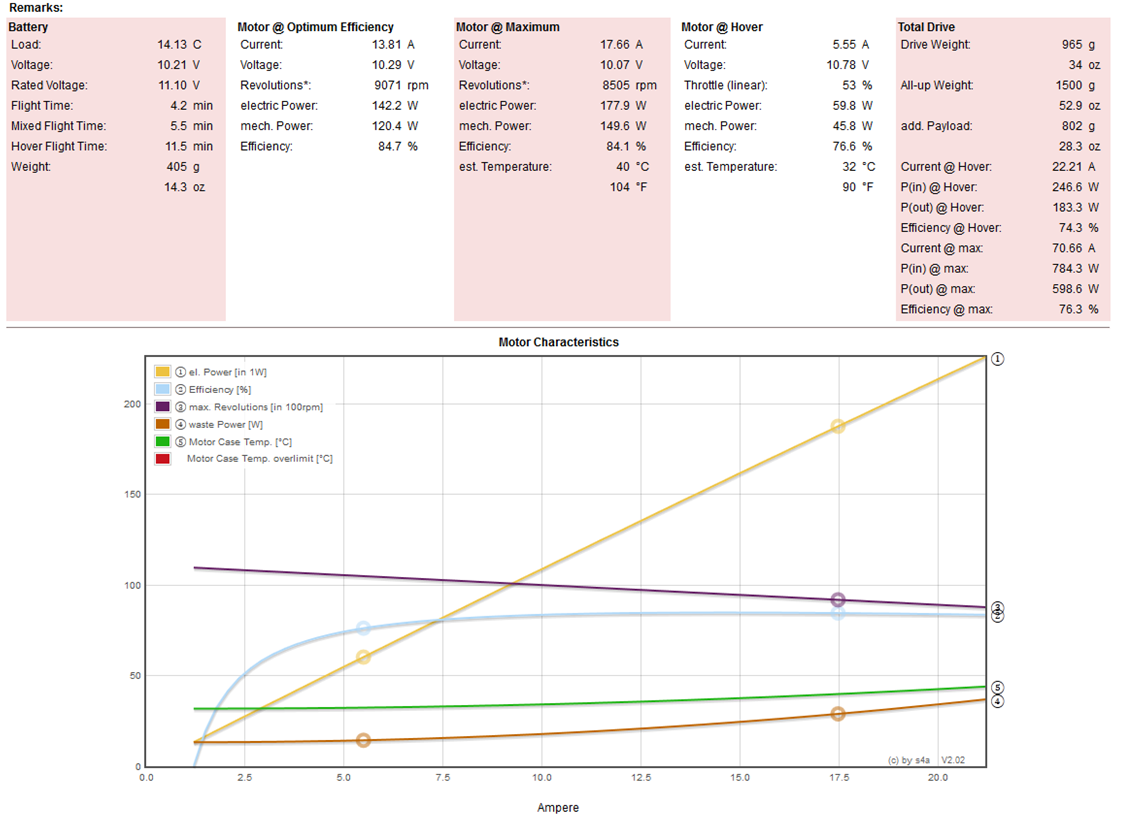
\includegraphics[width=1\textwidth]{Imatges/Componentes/10x4_5.png}
								\caption{Estudio con hélices de 10 pulgadas de diámetro y 4,5 pulgadas de paso}
								\label{fig:10inch}
							\end{figure}
							
					\item 11x4,5 (Figura \ref{fig:11inch})
					\begin{figure}
								\centering
								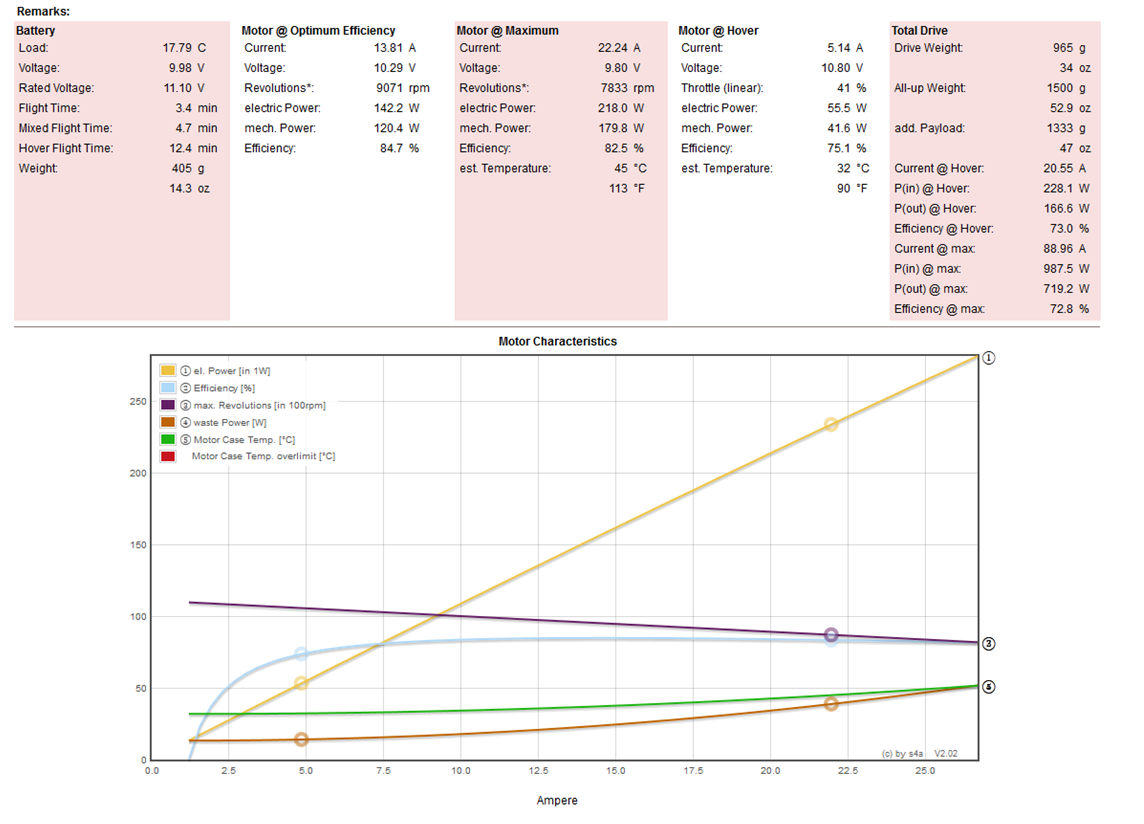
\includegraphics[width=1\textwidth]{Imatges/Componentes/11x4_5.png}
								\caption{Estudio con hélices de 11 pulgadas de diámetro y 4,5 pulgadas de paso}
								\label{fig:11inch}
							\end{figure}
							
					\item 12x4,5 (Figura \ref{fig:12inch})
					\begin{figure}
								\centering
								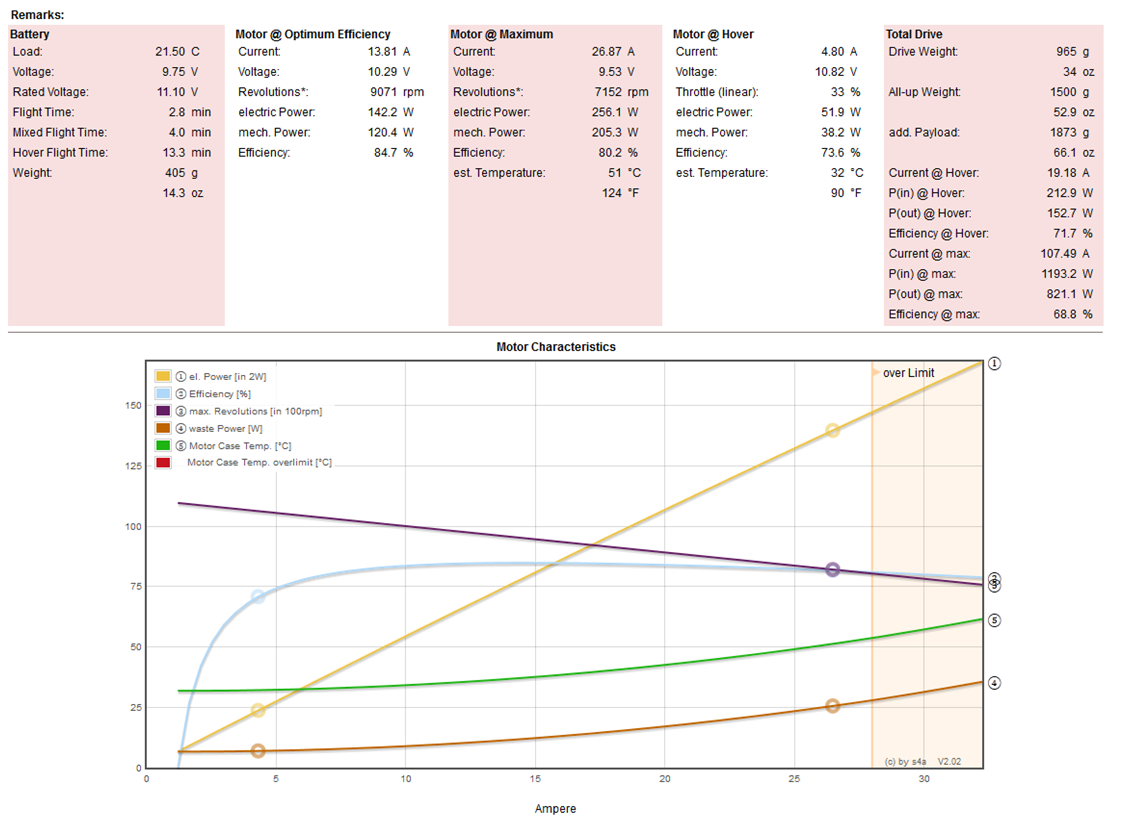
\includegraphics[width=1\textwidth]{Imatges/Componentes/12x4_5.png}
								\caption{Estudio con hélices de 12 pulgadas de diámetro y 4,5 pulgadas de paso}
								\label{fig:12inch}
							\end{figure}
				\end{itemize}
				
				\item ESC:
					
				Con las características de intensidad máxima del motor, $23,2A$, se ha decidido comprar variadores ESC de 30A (Figura \ref{fig:ESC_nuestro}), ya que es aconsejable tener un buen margen para los picos de corriente.
				
				\begin{figure}
					\centering
					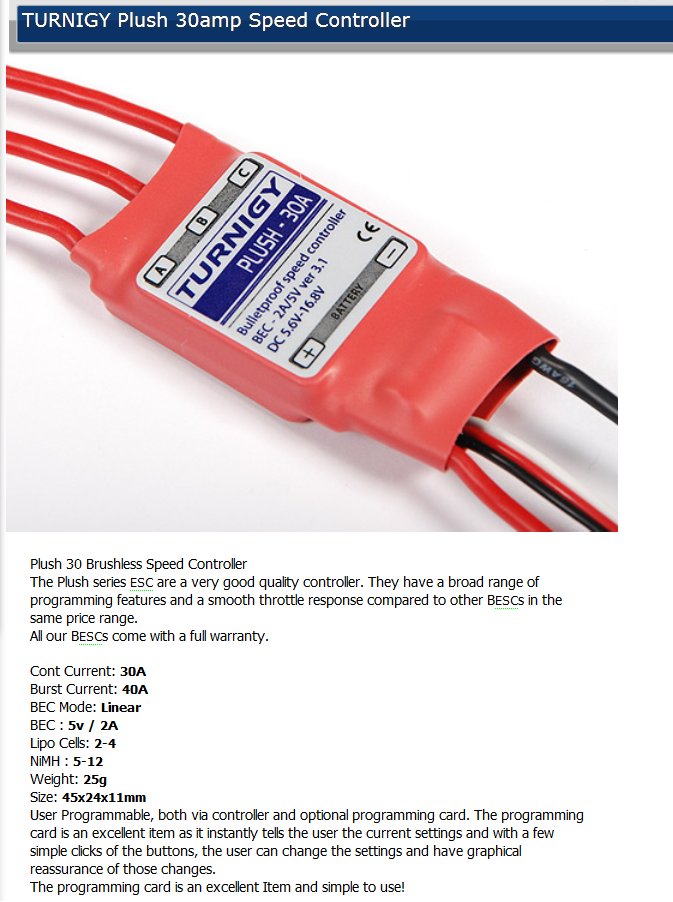
\includegraphics[width=0.8\textwidth]{Imatges/Componentes/ESC.png}
					\caption{Variador ESC escogido}
					\label{fig:ESC_nuestro}
			\end{figure}
				
			\end{itemize}
			
	\subsection{Elección del sistema de control y navegación}\label{subsec:control_navegacion}
	
		Para el sistema de control del cuadricóptero se ha elegido una IMU \textit{(Inercial Measurament Unit)} con 10 sensores (Figura \ref{fig:multiwii}). Se trata de un microcontrolador con acelerómetros (3 ejes), giroscopios (3 ejes), magnetómetros (3 ejes) y barómetro (1 eje). El microcontrolador recibe datos de todos los sensores, y los compara con los valores que quiere obtener. Con el error obtenido, mediante PIDs (control por realimentación Proporcional Integral Derivativo), intenta corregir el error obtenido y, por lo tanto, estabilizar el cuadricóptero en el aire.
		
		\begin{figure}
					\centering
					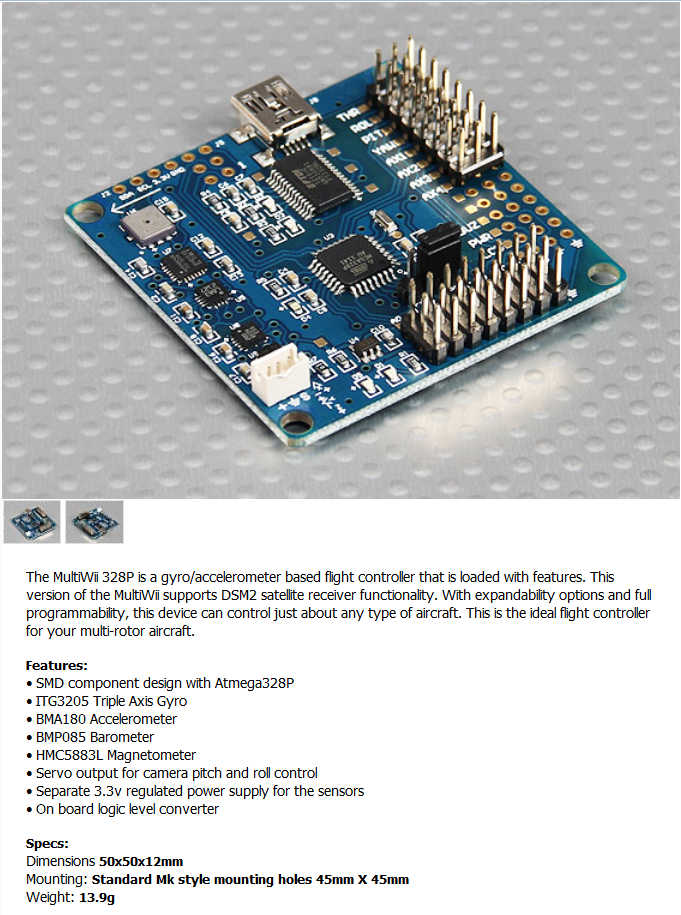
\includegraphics[width=0.8\textwidth]{Imatges/Componentes/multiwii.png}
					\caption{IMU elegida: MultiWii 328p}
					\label{fig:multiwii}
			\end{figure}
		
		El sistema de radio-control se realiza mediante una emisora de 9 canales y receptor de 8 canales (Figura \ref{fig:emisora}). Para controlar el cuadricóptero sólo se utilizan 4. Los otros servirán para configurar los modos de vuelo o otras funcionalidades cuando éste sea autónomo.
		
		\begin{figure}
					\centering
					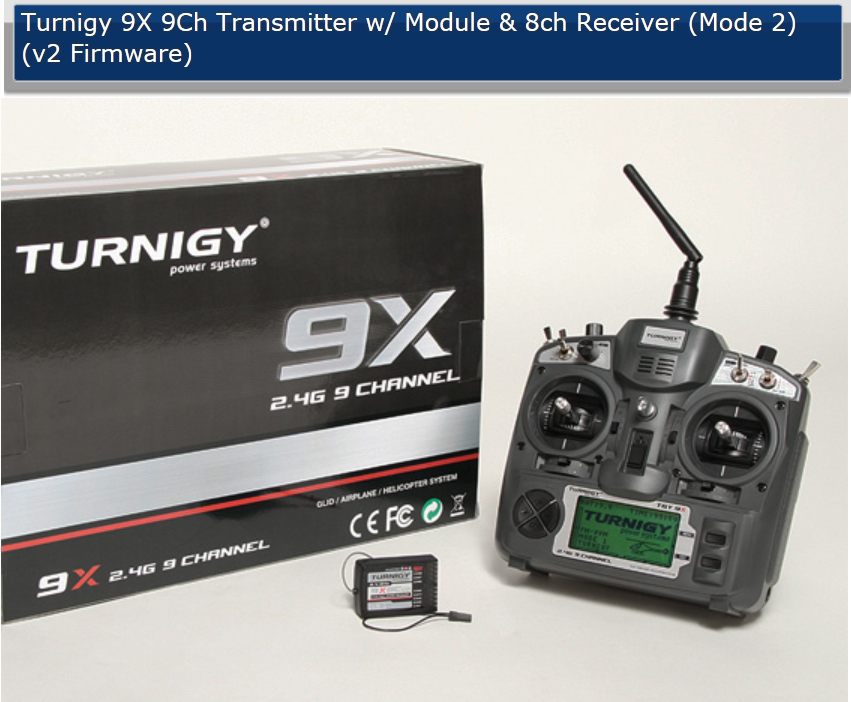
\includegraphics[width=0.8\textwidth]{Imatges/Componentes/emisora.png}
					\caption{Emisora escogida}
					\label{fig:emisora}
			\end{figure}
		
		Para la navegación se utilizará una Raspberry Pi (Figura \ref{fig:raspberry_pi}) con un sensor GPS, que gobernará al microcontrolador mediante un puerto serie.
		\begin{figure}
					\centering
					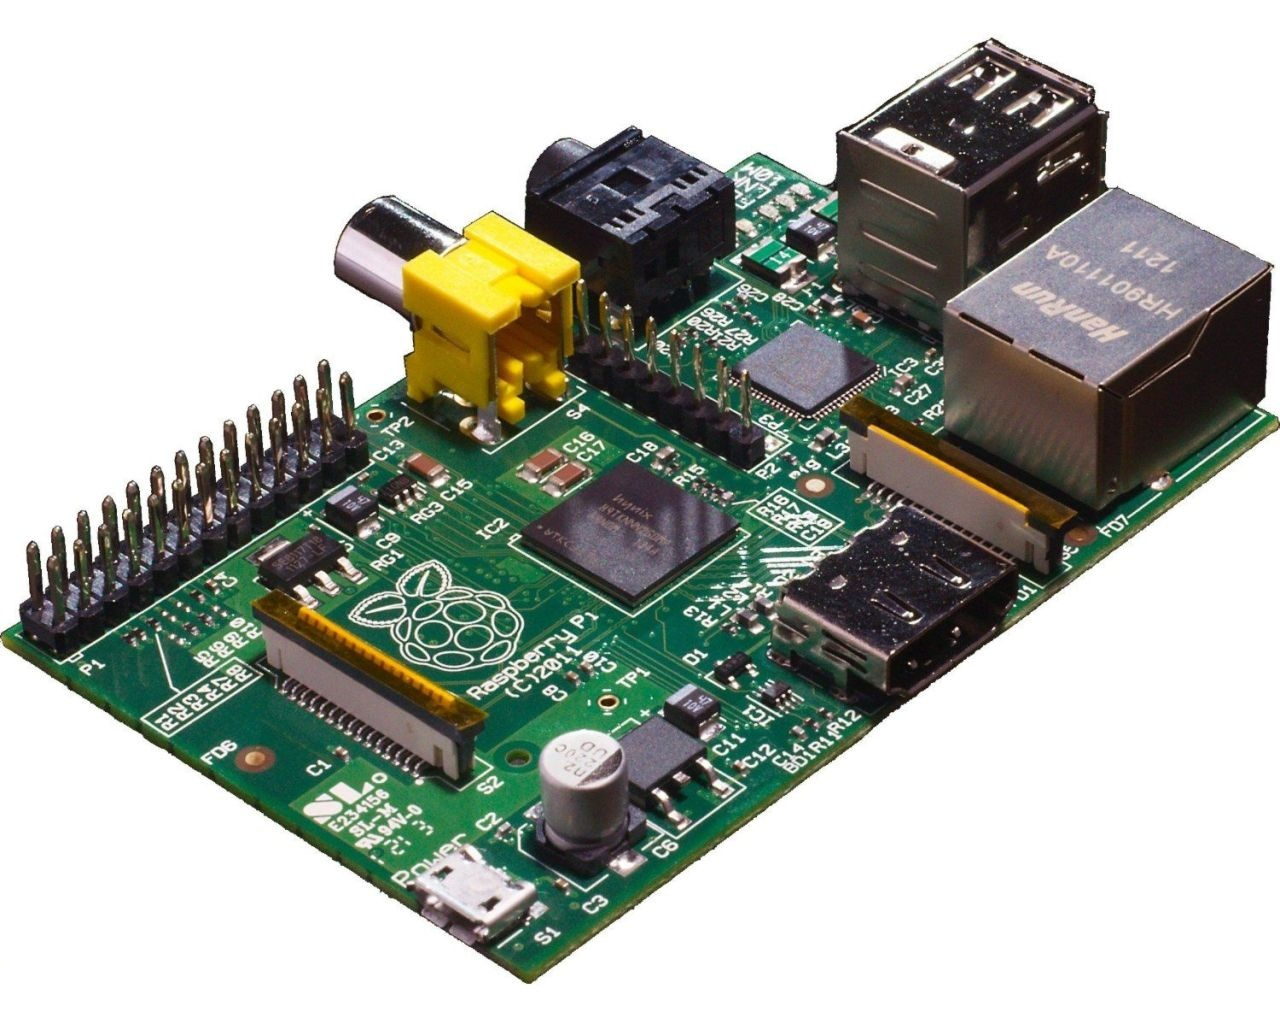
\includegraphics[width=0.8\textwidth]{Imatges/Componentes/raspberry_pi.jpg}
					\caption{Raspberry Pi}
					\label{fig:raspberry_pi}
			\end{figure}
		
	
  
\end{document}
